\documentclass[conference]{IEEEtran}
\usepackage{iftex}
\ifPDFTeX
\else
\usepackage{fontspec}
\setmainfont{TeX Gyre Termes}
\setsansfont{TeX Gyre Heros}
\setmonofont{TeX Gyre Cursor}
\fi
\usepackage{amsmath,amssymb,booktabs,array,multirow,enumitem,algorithm,algpseudocode,microtype,graphicx,pgfplots,placeins}
\usepackage{cite}
\usepackage[hidelinks]{hyperref}
\hypersetup{pdftitle={BaitFL: Lightweight Trap-Based Free-Rider Detection and Mitigation in Federated Learning},pdfauthor={Aashnan Rahman},pdfkeywords={federated learning,free-rider detection,robust statistics}}
\pgfplotsset{compat=1.18}
\usepgfplotslibrary{groupplots,fillbetween}
\definecolor{honestblue}{HTML}{2878A5}
\definecolor{riderorange}{HTML}{D66B27}
\providecommand*{\algorithmautorefname}{Algorithm}
\newcommand{\StudyRuns}{32}
\newcommand{\StudyTP}{1120}
\newcommand{\StudyFP}{0}
\newcommand{\StudyFN}{0}
\newcommand{\StudyHonest}{2080}
\newcommand{\StudyQuarantined}{11}
\newcommand{\StudyQuarantineRounds}{220}
\newcommand{\StudyCandidates}{296}

\newcommand{\MultiTP}{3360}
\newcommand{\MultiFP}{3}
\newcommand{\MultiFN}{0}
\newcommand{\MultiHonest}{6240}
\newcommand{\MultiQuarantined}{32}
\newcommand{\MultiCompletionMin}{30}
\newcommand{\MultiCompletionMax}{90}
\newcommand{\MultiPrecision}{99.91}
\newcommand{\MultiRecall}{100.00}
\newcommand{\MultiFone}{99.96}
\newcommand{\MultiMnistAccuracyMin}{98.83}
\newcommand{\MultiMnistAccuracyMax}{99.02}
\newcommand{\MultiCifarAccuracyMin}{74.51}
\newcommand{\MultiCifarAccuracyMax}{77.84}

\title{BaitFL: Lightweight Trap-Based Free-Rider Detection and Mitigation in Federated Learning}
\author{\IEEEauthorblockN{Aashnan Rahman}
\IEEEauthorblockA{Department of Computer Science and Engineering\\
Islamic University of Technology\\MSc Thesis}}
\begin{document}
\maketitle
\begin{tikzpicture}[remember picture,overlay]
\node[anchor=north east,font=\footnotesize] at ([xshift=-0.55in,yshift=-0.30in]current page.north east)
{Code v15.4 \textbar{} Paper v7 \textbar{} 30 October 2026};
\end{tikzpicture}

\begingroup\color{blue}
\begin{abstract}
\bfseries
Federated learning relies on participants performing useful local optimization,
but free riders can consume the shared model while submitting unchanged or
fabricated responses. Detecting such behavior is difficult when honest clients
have heterogeneous data and naturally different update statistics. This paper
investigates BaitFL, a server-side challenge protocol that compares responses to
undisclosed perturbations of the same model. Robust update-norm and tensor-profile
measurements first nominate anomalous clients; separate geometric separation
tests and repeated fresh evidence authorize removal. Component-specific memory
retains strong evidence across ambiguous cycles, while bounded quarantine
prevents weak suspicion from causing indefinite exclusion. The method requires
no auxiliary detector training, client-reported loss, or attack-specific history
reconstruction. We evaluate BaitFL across multiple random seeds on MNIST and
CIFAR-10, covering four fabrication strategies, IID and Dirichlet non-IID data,
and 30\% and 40\% free riders over 100 training rounds. The method achieves
\MultiRecall\% recall and pooled precision of \MultiPrecision\%. Most executions
complete removal at round 30, while difficult cases require up to
\MultiCompletionMax{} rounds. There are \MultiFP{} permanent honest-client
removals, and \MultiQuarantined{} honest client-cases experience temporary
quarantine. The findings support the approach under the evaluated settings.
Adaptive adversaries and secure aggregation remain outside the study's scope.
\end{abstract}
\endgroup
\begin{IEEEkeywords}
federated learning, free-rider detection, hidden challenges, robust statistics,
non-IID data, client auditing
\end{IEEEkeywords}

\section{Introduction}

Federated learning (FL) allows multiple clients to train a shared model
without handing over their local data. In each communication round, the
server distributes the current global model, the clients update it using
their own data, and the server aggregates the returned updates into a
revised model~\cite{mcmahan2017communication}. Since raw data stays with
its owner, FL is well suited to domains such as healthcare and personal
mobile services, where pooling sensitive records in one place is often
impractical or undesirable~\cite{rieke2020digitalhealth,mcmahan2017communication}.
This protection is not absolute, as shared updates can still leak
information~\cite{kairouz2021advances}. Exchanging updates instead of
datasets also avoids moving large volumes of local data, although repeated
model exchange remains a significant communication cost in
FL~\cite{mcmahan2017communication}. Effective collaboration depends on clients
performing useful local training, even though the server cannot directly
observe that work.

Like other distributed systems, FL is open to misconduct. Label-flipping and
model-poisoning attacks, for example, alter local data or submitted updates
in order to degrade the global model or introduce targeted
behavior~\cite{kairouz2021advances,bagdasaryan2020backdoor}. Free riding is
a quieter problem. The participant's primary aim is to obtain the shared
model without paying the cost of local
training~\cite{lin2019freeriders,fraboni2021freerider}. A client may lack
useful data or computational resources, or may simply choose to conserve
them. Instead of training, it can return an unchanged model, fabricate a
noisy response, or build an update from models received in earlier rounds.
Such responses may resemble what the server expects, so they need not
visibly disrupt learning and can evade checks aimed at overtly harmful
updates. Free riding shifts the training burden to honest participants. When
a client withholds useful data and computation, the federation also loses a
contribution that could have improved the shared model.

Detecting this omission is difficult because unusual updates are not limited
to free riders. Honest clients differ in sample sizes, class distributions,
and local learning trajectories, particularly under non-IID
data~\cite{kairouz2021advances}. A small update can therefore reflect
legitimate training, while a fabricated one can look like an ordinary
contribution. The server has to tell these cases apart without observing
local optimization. Existing approaches rely on learned anomaly models,
parameter audits, or evidence obtained through inference
attacks~\cite{lin2019freeriders,wang2024pass,recasens2026frida}. This raises a
practical question: can lightweight server-side checks detect free riding
without training an auxiliary detector? There is also a cost to being wrong.
Withholding an honest client's updates can reduce its contribution to the shared
model, even if it is never permanently removed. A detector must therefore
consider both the evidence needed for removal and the duration of temporary
exclusion.

To address this problem, we propose \emph{BaitFL}, a lightweight trap-based
method for detecting and mitigating free riders in federated learning.

\noindent{The main contributions of this work are as follows:}
\begin{itemize} %[leftmargin=*,nosep]
\item \textbf{Lightweight server-side detection.} We develop a challenge-based
detector using update norms and tensor profiles, without training an auxiliary
detection model or accessing clients' private training data.
\item \textbf{Confirmation using repeated evidence.} We design a decision
mechanism that separates initial suspicion from permanent removal and requires
fresh evidence of the same component across two challenges and distinct audit
cycles for statistical confirmation.
\item \textbf{Bounded mitigation and rehabilitation.} We retain strong evidence
across ambiguous cycles while allowing unconfirmed quarantine to expire and
clearing statistical memory after repeated clean observations.
\item \textbf{Evaluation across four free-rider behaviors.} We study unchanged-model
responses, random fabrication, history averaging, and trajectory imitation on
MNIST and CIFAR-10 under IID and non-IID partitions, with 30\% and 40\% free riders.
\end{itemize}

The remainder of the paper reviews related work, defines the threat model
and the free-rider behaviors evaluated, describes the auditing method in
detail, and reports the resulting detection performance, computational cost,
and limitations.

% Literature review is retained in the author's current black text.
\section{Literature Review}
\subsection{Free-Rider Attacks and Evasion}
Lin \emph{et al.} studied clients that fabricate updates without local training
data, including random submissions and responses derived from changes in the
global model~\cite{lin2019freeriders}. They showed that taking part in model
exchange does not establish taking part in training. The evaluated fabrications
were detectable, but this does not guarantee that every non-training client
will remain distinguishable from honest clients.

Fraboni \emph{et al.} analyzed free riding under iterative model aggregation
and developed stochastic disguises that follow the trajectory of the shared
model~\cite{fraboni2021freerider}. Their analysis showed that a free rider can
approach the model obtained by contributing participants, which makes simple
unchanged-model checks insufficient. Zhu \emph{et al.} analyzed local and
global training dynamics with an Ornstein--Uhlenbeck model and proposed
scaled-delta and advanced free-rider attacks that address both convergence and
stealth~\cite{zhu2021advanced}. These attacks expose a weakness of passive
update screening, since a fabricated update can be designed to match the
statistics a detector observes. This motivates auditing responses to
controlled challenges instead of relying only on how ordinary updates look.

\subsection{Learned Detection and Contribution Auditing}
To detect fabricated updates, Lin \emph{et al.} proposed STD-DAGMM, which
combines an autoencoder-based representation, reconstruction information, and
update standard deviation with mixture-based anomaly
scoring~\cite{lin2019freeriders}. Adding the standard deviation improved
separation for attacks that the original DAGMM detector struggled with. This
gives richer evidence than a single scalar statistic, but it requires fitting
an auxiliary encoder, decoder, and estimation network on high-dimensional
updates. Training and storing this additional model adds computation and
memory cost that compact update summaries avoid.
Section~\ref{sec:native-timing} reports the fitting cost measured in our
STD-DAGMM implementation.

Wang \emph{et al.} proposed FRAD for AIoT, which combines DAGMM with
contribution and reputation information~\cite{wang2024frad}. Contribution is
modeled from computing resources, communication cost, and data quality, and a
PageRank-based reputation guides participant selection. This extends anomaly
detection with historical evidence, and the authors report detection under high
free-rider proportions. FRAD still fits an auxiliary detector, however, and it
needs resource and quality signals beyond the returned model updates, which are
an extra deployment requirement to obtain reliably. Contribution ranking alone
also cannot tell whether a low-ranked client skipped training.

Separately, Wang \emph{et al.} introduced PASS, in which clients audit other
participants' updates on their own private datasets and return accuracy-based
contribution scores~\cite{wang2024pass}. PASS addresses both anonymous and
selfish free riders, including evaluated settings where attackers are the
majority. Peer auditing, however, adds local model evaluation, update
distribution, and score reporting. It also gives clients access to individual
updates, a privacy exposure that PASS mitigates with Gaussian perturbation and
parameter pruning, at the price of reduced audit utility. The authors leave
network-cost validation open, since their standalone simulator does not
measure communication. In addition, an accuracy-based score depends on the
evaluator's data, so under heterogeneity low utility and absence of training
need not coincide.

\subsection{Canary-Based Evidence and Privacy Tradeoffs}
Recasens \emph{et al.} proposed FRIDA, which repurposes membership and property
inference to obtain evidence that a client trained~\cite{recasens2026frida}.
Its membership-based variants ask clients to train on server-provided canary
examples and assess the effect through loss or gradient similarity. This
creates an explicit training signal rather than relying on incidental update
statistics. Canary construction and distribution, though, require additional
labeled examples, canary training adds client work beyond the original local
task, and loss or gradient testing adds server computation. The signal also
shows that the canary task was used, not that the client's private data
contributed useful work.

FRIDA's property-based variants infer characteristics such as local label
distributions and test their consistency or diversity~\cite{recasens2026frida}.
They avoid canary training but deliberately extract information about local
data, which may itself be sensitive. The two families therefore carry different
costs: extra training on challenge data for membership tests, and disclosure of
inferred dataset properties for property tests.

Secure aggregation, developed by Bonawitz \emph{et al.}, combines client
updates without revealing them individually~\cite{bonawitz2017practical}. This
protects individual contributions but conflicts with detectors that need
attributable responses. BaitFL shares this limitation. Avoiding raw-data access
and property inference does not make individual model responses private, and
the method cannot be inserted unchanged into standard secure aggregation.

Taken together, these limitations point to three practical requirements: less
auxiliary detector training, no additional client-side evaluation or canary
tasks, and a clear separation between suspicion and sufficient evidence for
removal. BaitFL studies model perturbations and repeated evidence from update
norms and tensor profiles under these requirements. Its challenge rounds still
consume client work and withhold responses from aggregation, so execution cost
and honest-client exclusion must be evaluated alongside detection quality.


\color{black}

\section{Threat Model}
\subsection{Participants and Server Knowledge}
We consider a trusted server coordinating $N$ clients with persistent identities
and reliable communication. All active clients respond in every round, with no
client sampling, late arrivals, or dropouts. Removed clients no longer
participate. Quarantined clients continue to respond. Their responses and all
responses to traps are excluded from aggregation. Honest clients train the
model they receive using the prescribed optimizer. Their local data may differ
in size and class distribution, and the experiments cover both IID and non-IID
partitions.

The server can send different model states to different clients. Clients are
not told whether the model they receive is an ordinary global model or a trap.
For client $i$ in round $t$, the server knows the model it sent,
$w^{\rm send}_{t,i}$, and the model returned by the client,
$w^{\rm ret}_{t,i}$. It computes the update and its norm as
\begin{equation}
 \Delta_{t,i}=w^{\rm ret}_{t,i}-w^{\rm send}_{t,i},\qquad
 r_{t,i}=\|\Delta_{t,i}\|_2.
\end{equation}
Screening uses the returned models and the server's audit history. It does not
require private training records or prior knowledge of which clients are free
riders or how they fabricate their responses. The server observes individual
client responses, so this setting does not use secure aggregation.

\subsection{Free-Rider Objective and Scope}
The free riders considered here seek access to the shared model without
performing local training. A client may have no suitable data, lack the resources
needed to train the model, or possess both but choose not to use them. It can
still receive and store models and perform the relatively simple calculations
needed to fabricate a response. Its objective is to avoid training costs rather
than to introduce a targeted error or backdoor into the global model.

We study persistent free riding: a free rider performs no local optimization
at any stage of an experiment. Clients that train for fewer local steps or
alternate between honest training and free riding are outside this scope.
Each free rider uses only its own received-model history and local randomness.
Free riders do not collude, share responses, or change identities. Their response
strategies do not adapt to identify or evade audits. Adaptive strategies and
the possibility of recognizing traps are discussed in
Section~\ref{sec:evasion}.

We assume an honest majority because the detector uses robust peer statistics
as its reference and seeks a separated minority of suspicious responses.
The experiments use 30\% and 40\% free riders. Each experiment evaluates one
fixed fabrication strategy for all free riders. The four strategies are defined
below.

\subsection{Evaluated Free-Rider Behaviors}
For a free rider, the returned model is $w^{\rm ret}_{t,i}=\widehat w_{t,i}$.
The following equations apply to floating entries of the model state, including
floating buffers. Integer entries are copied unchanged from the received model.

\noindent\textbf{FR1: current-model sendback.}
The client returns the received model unchanged,
\begin{equation}
 \widehat w_{t,i}=w^{\rm send}_{t,i}.
\end{equation}
This produces a zero update without local training, regardless of whether the
received model is a trap.

\medskip\noindent\textbf{FR2: bounded random fabrication.}
The client adds independent uniform noise to each floating point entry of the
received model state,
\begin{equation}
 \widehat w_{t,i}=w^{\rm send}_{t,i}+\epsilon_{t,i},\quad
 (\epsilon_{t,i})_j\sim\mathcal U(-10^{-3},10^{-3}).
\end{equation}
The added noise makes the response differ from the received model without
performing any local training.

\medskip\noindent\textbf{FR3: received-history averaging.}
Let $H$ be the history length and $\mathcal H_{t,i}$ contain the most recent
$\min(H,t)$ model states received by client $i$. The client returns their mean,
\begin{equation}
 \widehat w_{t,i}=\frac{1}{|\mathcal H_{t,i}|}
       \sum_{w\in\mathcal H_{t,i}}w.
\end{equation}
The history includes the current model and any traps received during earlier
rounds. Averaging these states produces a response based on the shared model's
recent evolution without using local training data.

\medskip\noindent\textbf{FR4: received-trajectory imitation.}
The client computes differences between consecutive received models,
\begin{equation}
 d_{s,i}=w^{\rm send}_{s,i}-w^{\rm send}_{s-1,i}.
\end{equation}
Let $\overline d_{t,i}$ be the mean of up to five most recent differences.
The response is
\begin{equation}
 \widehat w_{t,i}=w^{\rm send}_{t,i}+\overline d_{t,i}+\eta_{t,i}.
\end{equation}
Once differences are available, the client draws a standard Gaussian vector
$z_{t,i}$ and rescales it to obtain
\begin{equation}\label{eq:fr4-noise}
 \eta_{t,i}=0.1\,
 \frac{\max(\|\overline d_{t,i}\|_2,\epsilon_0)}
      {\max(\|z_{t,i}\|_2,\epsilon_0)}\,z_{t,i},
 \qquad\epsilon_0=10^{-6}.
\end{equation}
These vectors contain all floating model entries. For its first response,
$\overline d_{1,i}=0$ and $\eta_{1,i}$ instead has independent Gaussian
coordinates with standard deviation $10^{-4}$. Received traps enter the
difference history just like ordinary models, so they also affect the estimated
trajectory. This strategy follows recent model changes while adding variation
to the fabricated response.

\section{Proposed Methodology}
BaitFL audits clients by observing how they respond to perturbed models. The
procedure has four phases: warmup, initial paired coverage, confirmation and
review, and sparse auditing. Update statistics identify clients for further
checks. Permanent removal requires repeated evidence, while temporary exclusion
has a separate review budget. The client records $\mathcal S$ store each client's
status, evidence, and review progress.

\subsection{Challenges, Measurements, and Aggregation}
At the start of a paired audit cycle, the server takes a copy $w^{(c)}$ of the
current global model and creates two traps, $A$ and $B$. For floating tensor
$k$, trap $a\in\{A,B\}$ is
\begin{equation}\label{eq:trap}
 \tau_{a,k}=w^{(c)}_k+
 \gamma\max\{\operatorname{sd}(w^{(c)}_k),\epsilon_\tau\}\xi_{a,k},
 \quad\xi_{a,k}\sim\mathcal N(0,I).
\end{equation}
The two traps use independent noise. We set $\gamma=0.01$ and
$\epsilon_\tau=10^{-4}$. Perturbations apply to floating model tensors,
including BatchNorm buffers. Integer counters are unchanged. Both traps remain
fixed for the cycle, even as ordinary updates change the global model.

For each response, the server records the update norm $r_i$ and a tensor profile
$p_i$. Its coordinate for tensor $k$ is
\begin{equation}\label{eq:profile}
 p_{i,k}=\frac{\|\Delta_{i,k}\|_2}{\sum_j\|\Delta_{i,j}\|_2}.
\end{equation}
When the denominator is below $10^{-6}$, the profile is set to zero. The norm
measures update magnitude, while the profile describes how that magnitude is
distributed across model tensors.

Clients are compared only with others that received the same trap. The reference
for client $i$ consists of all other active clients with a response to that trap.
Let $m_i$ be the median of their update norms and $d_i$ the median absolute
deviation. The normalized norm score is
\begin{equation}\label{eq:norm-score}
 z_i^n=\frac{r_i-m_i}{d_i/\Phi^{-1}(0.75)},
\end{equation}
where $\Phi$ is the standard normal cumulative distribution function. For the
profile score, the server first forms the coordinatewise median of the peer
profiles. It measures each profile's Euclidean distance from that reference and
normalizes the client's distance using the median and median absolute deviation
of the peer distances. This gives $z_i^p$. A zero median absolute deviation leaves
the corresponding score undefined.

Only ordinary responses from eligible clients enter aggregation. Let
$\mathcal A_t$ be the clients that were neither trapped nor quarantined during
round $t$, after excluding any clients removed or newly quarantined at its end.
The aggregation routine used in the algorithms is
\begin{equation}\label{eq:method-aggregation}
 w_{t+1}=w_t+\frac{1}{|\mathcal A_t|}
                 \sum_{i\in\mathcal A_t}\Delta_{t,i}.
\end{equation}
If $\mathcal A_t$ is empty, the model is unchanged. Clients receive equal
weight. Training on a trap replaces ordinary local training for that round.

\subsection{Phase I: Warmup}
The first ten rounds use the ordinary global model. Clients return their
responses and the server aggregates them, as shown in
Algorithm~\ref{alg:warmup}, lines~\ref{ln:warm:send} to~\ref{ln:warm:aggregate}.
This gives the federation an initial training trajectory before audits begin.
Client evidence counters start at zero, and no client is removed during warmup.

\begin{algorithm}[t]
\caption{Phase I: ordinary training during warmup}\label{alg:warmup}
\begin{algorithmic}[1]\small
\Procedure{Warmup}{$w,\mathcal S$}
 \For{$t=1,\ldots,10$}
  \State Send $w$ to all active clients\label{ln:warm:send}
  \State Collect responses and record their update summaries
  \State $\mathcal A_t\gets$ all active clients
  \State $w\gets\Call{Aggregate}{w,\mathcal A_t}$\label{ln:warm:aggregate}
 \EndFor
 \State \Return $(w,10,\mathcal S)$
\EndProcedure
\end{algorithmic}
\end{algorithm}

\subsection{Phase II: Initial Paired Coverage}
Rounds 11 to 20 give every client one response to each trap. The server shuffles
clients into at most ten groups. It assigns pairs of groups to traps during the
first half of the cycle, then repeats the assignments with the opposite trap.
With 100 clients, approximately 20\% receive a trap in each round. The remaining
clients receive the current global model.

Algorithm~\ref{alg:paired} describes this collection procedure and its reuse in
later confirmation cycles. The server chooses one response position for each
client and trap before observing the responses, as shown on
line~\ref{ln:paired:select}. It waits for the complete pair before making a cycle
decision on lines~\ref{ln:paired:screen} to~\ref{ln:paired:confirm}. The last
round's aggregation follows that decision so newly excluded responses do not
enter the global model.

\subsubsection{Screening}
The server calculates $D_i=z_i^p-z_i^n$ for trap $A$, trap $B$, and their average.
For each view, it builds a histogram with $\lceil\sqrt{n_v}\rceil$ equally spaced
bins, where $n_v$ is the number of clients with valid paired scores. An Otsu split
provides a boundary between the two score groups~\cite{otsu1979threshold}.
The split is accepted only when the lower side of the averaged view contains
a majority of active clients. The server then uses 1,000 bootstrap samples to
estimate a 99\% interval for each boundary~\cite{efron1979bootstrap}. The same
resampled clients are used in all three views.

A client above the upper boundary in every view is nominated as suspicious.
One below the lower boundary in every view is clear. The remaining clients are
candidates for further checking. If a usable split cannot be obtained, norms
below the peer median on both traps nominate suspicion. Neither norm below the
median gives a clear result. A single low norm or an undefined score gives a
candidate result.

\subsubsection{Geometric evidence}
Suspicion must pass an additional separation test before it counts toward
removal. On each trap, let $\mathcal C$ be the nominated cohort and $\mathcal P$
the remaining clients. With $n$ active clients, the cohort must satisfy
\begin{equation}\label{eq:cohort-support}
 \left\lceil\frac{n}{\lceil\sqrt n\rceil}\right\rceil
       \leq|\mathcal C|<|\mathcal P|.
\end{equation}
Quartiles are calculated separately for norms and profile distances.
Write $Q_q(\mathcal C)$ for the empirical quantile at level $q$ and
$I_C=Q_{.75}(\mathcal C)-Q_{.25}(\mathcal C)$ for its interquartile range.
For low update norms, evidence is accepted when
\begin{align}\label{eq:norm-certificate}
 Q_{.25}(\mathcal P)-Q_{.75}(\mathcal C)&>I_C,\\
 \min(\mathcal P)-Q_{.75}(\mathcal C)&>I_C.\nonumber
\end{align}
A nominated client must also have a norm below the median of $\mathcal P$.
These conditions require separation from the peer population, rather than
concentration within the nominated group alone.

For high profile distances, define
$I_P=Q_{.75}(\mathcal P)-Q_{.25}(\mathcal P)$ and
$g=Q_{.25}(\mathcal C)-Q_{.75}(\mathcal P)$. Evidence requires $g>I_C$,
$g>0$, and either
\begin{equation}\label{eq:profile-certificate}
 Q_{.25}(\mathcal C)-\max(\mathcal P)>I_C
 \quad\text{or}\quad
 \frac{I_C}{|\mathcal C|-1}<\frac{I_P}{|\mathcal P|-1}.
\end{equation}
The client's distance must exceed the median of $\mathcal P$. A norm or profile
certificate is recorded only when the same component supports that client on
both traps. Exact copies of the current or immediately preceding sent model
are recorded separately on each trap.

After these checks, $S$ denotes strong paired evidence, $C$ denotes an unresolved
candidate, and $R$ denotes a clear cycle result. Only a paired geometric
certificate contributes to statistical confirmation. The routine
\textsc{ScreenAndCertify} in
Algorithm~\ref{alg:paired} applies these rules and returns the component
certificates, exact replay flags, and cycle outcomes.

\begin{algorithm}[t]
\caption{Phase II: collect a complete pair of trap responses}\label{alg:paired}
\begin{algorithmic}[1]\small
\Require Training horizon $T$
\Procedure{PairedCycle}{$w,t,\mathcal S,\mathrm{initial}$}
 \State Advance the cycle number $c$
 \State Create $\tau_A,\tau_B$ from $w$ using Eq.~\eqref{eq:trap}
 \If{$\mathrm{initial}$}
  \State Shuffle clients into groups and schedule paired coverage
 \Else
  \State Separate clients under review from ordinary clients
  \State Schedule alternating traps for reviewed clients
  \State Give ordinary clients one response to each trap
 \EndIf
 \State Preselect one position per client and trap\label{ln:paired:select}
 \State Initialize selected observations $O$
 \State $L\gets\min(10,T-t)$
 \For{$s=1,\ldots,L$}
  \State $t\gets t+1$
  \State Read the scheduled trap and recipient set $\mathcal T_t$
  \State Send the trap to $\mathcal T_t$ and $w$ to other clients
  \State Collect responses and store the preselected observations
  \State $\mathcal A_t\gets$ ordinary clients not quarantined at round start
  \If{$s=10$}
   \State $E\gets\Call{ScreenAndCertify}{O}$\label{ln:paired:screen}
   \State $\mathcal S\gets\Call{Confirm}{\mathcal S,E,c}$\label{ln:paired:confirm}
   \State Exclude new removals and quarantines from $\mathcal A_t$
  \EndIf
  \State $w\gets\Call{Aggregate}{w,\mathcal A_t}$
 \EndFor
 \State Update the audit clock from the remaining review state
 \State \Return $(w,t,\mathcal S)$
\EndProcedure
\end{algorithmic}
\end{algorithm}

\subsection{Phase III: Confirmation and Bounded Review}
The server keeps separate certificate counts $M_{i,n}$ and $M_{i,p}$ for each
client. A fresh paired certificate increases its own count once in a completed
cycle. Ambiguous cycles retain the counts. Two consecutive clear cycles erase
them. Statistical removal requires a fresh certificate whose component count
reaches two, as shown in Algorithm~\ref{alg:confirmation},
lines~\ref{ln:confirm:increment} to~\ref{ln:confirm:remove}. Norm evidence in one
cycle and profile evidence in another do not confirm one another. Exact replay
uses a separate rule that requires evidence on both traps in two consecutive
completed cycles. With the ten warmup rounds and ten rounds per paired cycle,
the earliest removal is at round 30.

A fresh strong result places the client in quarantine and starts a review budget
of two cycles. Another fresh strong result renews that budget. Otherwise, it
decreases after each completed cycle. When the budget expires, the client is
released even if unresolved evidence remains in memory. A candidate without
strong evidence may contribute on ordinary rounds. Two consecutive clear
results rehabilitate a suspected or candidate client. One additional clear
cycle completes probation before routine auditing resumes. Clients released
from unresolved review have a cooldown of two sparse audits before weak
evidence can enroll them again. Fresh paired evidence can still start review.

During confirmation, reviewed and ordinary clients are grouped separately.
At most ten groups are allocated in proportion to the two populations.
Reviewed clients receive alternating traps throughout the cycle. Ordinary
clients receive each trap once. As in the initial cycle, the decision uses only
the response positions selected in advance. Each new cycle creates fresh traps.
Algorithm~\ref{alg:paired} collects these responses, and
Algorithm~\ref{alg:confirmation} updates the client records at the cycle boundary.

\begin{algorithm}[t]
\caption{Phase III: confirm evidence and manage review}\label{alg:confirmation}
\begin{algorithmic}[1]\small
\Procedure{Confirm}{$\mathcal S,E,c$}
 \ForAll{active clients $i$}
  \State $J_i\gets$ components certified on both traps in $E$
  \State Update the consecutive paired exact replay count
  \If{$J_i\ne\emptyset$}
   \ForAll{$j\in J_i$}
    \State $M_{i,j}\gets M_{i,j}+1$\label{ln:confirm:increment}
   \EndFor
   \State Reset the consecutive clear cycle count
  \ElsIf{the cycle outcome is $R$}
   \State Advance the consecutive clear cycle count
   \If{two consecutive clear cycles are complete}
    \State $M_{i,n}\gets0$, $M_{i,p}\gets0$
   \EndIf
  \Else
   \State Reset the clear cycle count and retain certificate memory
  \EndIf
  \If{a fresh component count reaches two or exact replay is confirmed}
   \State Permanently remove $i$\label{ln:confirm:remove}
  \ElsIf{$J_i\ne\emptyset$ or paired exact replay is present}
   \State Quarantine $i$ and set its review budget to two cycles
   \State Reset its clean progress, probation, and cooldown
  \Else
   \State Decrease the review budget toward zero
   \State Apply clear cycle rehabilitation and probation
   \If{unconfirmed review has just expired}
    \State Release $i$ and set a cooldown of two sparse audits
   \EndIf
  \EndIf
 \EndFor
 \State \Return $\mathcal S$
\EndProcedure
\end{algorithmic}
\end{algorithm}

\subsection{Phase IV: Sparse Audits}
When no client remains under review or probation, the server returns to ordinary
training and schedules a sparse audit after ten rounds. In an audit round,
all active clients receive the same fresh trap, so the global model remains
unchanged for that round. Ordinary rounds between audits use
Eq.~\eqref{eq:method-aggregation}.

The audit applies the same norm and profile measurements to one trap. Screening
nominates a cohort, and the geometric tests identify clients for further review.
Exact replay also triggers review. Algorithm~\ref{alg:sparse},
lines~\ref{ln:sparse:measure} to~\ref{ln:sparse:enroll}, shows this step.
Eligible clients enter a two cycle review without immediate quarantine.
The server then resumes paired cycles. A sparse audit cannot increase
statistical certificate counts, clear certificate memory, or authorize removal.

\begin{algorithm}[t]
\caption{Phase IV: ordinary training and sparse auditing}\label{alg:sparse}
\begin{algorithmic}[1]\small
\Procedure{SparseRound}{$w,t,\mathcal S$}
 \State $t\gets t+1$
 \If{a sparse audit is due}
  \State Create a fresh trap and send it to all active clients
  \State Collect responses and compute norm and profile scores\label{ln:sparse:measure}
  \State $\mathcal F\gets$ clients selected by geometric evidence or exact replay
  \State Identify clients currently in audit cooldown
  \State Decrease audit cooldowns toward zero
  \ForAll{$i\in\mathcal F$ not in the identified cooldown set}
   \State Open two cycles of review without quarantine\label{ln:sparse:enroll}
   \State Reset clean progress and consecutive exact replay evidence
  \EndFor
  \State Update the audit clock from the screening outcome
 \Else
  \State Send $w$ to all active clients and collect responses
  \State $\mathcal A_t\gets$ ordinary clients not quarantined
  \State $w\gets\Call{Aggregate}{w,\mathcal A_t}$
 \EndIf
 \State \Return $(w,t,\mathcal S)$
\EndProcedure
\end{algorithmic}
\end{algorithm}

\subsection{Overall Procedure}
Algorithm~\ref{alg:baitfl} connects the four phases. The client records
$\mathcal S$ contain membership, quarantine and review status, certificate
counts, clean progress, probation, and cooldowns. After warmup, every client
receives initial paired coverage. Further paired cycles run while review or
probation is pending. Otherwise, the server uses ordinary training with sparse
audits until the training horizon is reached.

\begin{algorithm}[t]
\caption{Overall BaitFL procedure}\label{alg:baitfl}
\begin{algorithmic}[1]\small
\Require Initial model $w$, clients, training horizon $T\geq30$
\State Initialize client records $\mathcal S$ and zero evidence counts
\State $(w,t,\mathcal S)\gets\Call{Warmup}{w,\mathcal S}$
\State $\mathrm{initial}\gets\mathrm{true}$
\While{$t<T$ and active clients remain}
 \If{$\mathrm{initial}$ or review or probation is pending}
  \State $(w,t,\mathcal S)\gets\Call{PairedCycle}{w,t,\mathcal S,\mathrm{initial}}$
  \State $\mathrm{initial}\gets\mathrm{false}$
 \Else
  \State $(w,t,\mathcal S)\gets\Call{SparseRound}{w,t,\mathcal S}$
 \EndIf
\EndWhile
\State \Return $w$ and the final client records $\mathcal S$
\end{algorithmic}
\end{algorithm}

\FloatBarrier
% Results and later sections remain red for revision.
\color{red}

\section{Results}
\subsection{Experimental Setup}
We evaluate BaitFL on MNIST and CIFAR-10, which contain handwritten digit
images and color images from ten object classes,
respectively~\cite{lecun1998gradient,krizhevsky2009learning}. The evaluation
covers four free-rider behaviors, IID and non-IID client data, and free-rider
proportions of 30\% and 40\%. Each configuration is repeated using multiple
random seeds, and Table~\ref{tab:performance} reports the corresponding mean
performance. The optimizer and detector settings remain fixed across
replications.

Each federation contains 100 clients and trains for 100 communication rounds.
For IID experiments, data are randomly divided into client partitions of equal
size. For non-IID experiments, class proportions are allocated using a Dirichlet
distribution with $\alpha=0.5$, with allocation repeated if a client receives
no samples. Replications vary data partitioning, attacker assignment, model
initialization, training randomness, and audit scheduling.

Honest clients perform three local SGD epochs per round with learning rate
0.01, momentum 0.9, and batch size 32. FR3 uses history length $H=5$.
The MNIST model has two convolutional blocks with 16 and 32 channels and a
128-unit hidden classifier. The CIFAR-10 model has three convolutional blocks
with BatchNorm and 32, 64, and 128 channels, followed by a 256-unit hidden
classifier. Images are normalized without data augmentation, and all experiments
use CPU execution.

\subsection{Evaluation Metrics}
A positive detection is \emph{permanent removal}, not nomination or quarantine.
For true positives $TP$, honest removals $FP$, and missed free riders $FN$,
\begin{equation}
 \begin{aligned}
 P&=\frac{TP}{TP+FP},\qquad R=\frac{TP}{TP+FN},\\
 F_1&=\frac{2TP}{2TP+FP+FN}.
 \end{aligned}
\end{equation}
Precision is undefined if no client is removed. Complete-detection round
$t_{\rm all}$ exists only when every free rider has been removed; otherwise it
is NR. Final global test accuracy is a separate utility metric. We additionally
report final honest-candidate counts, honest clients ever quarantined, quarantine
client-rounds, trap client-rounds, and all excluded active honest client-rounds.
These last categories can overlap and must not be summed as disjoint costs.

\subsection{Permanent Detection and Model Utility}
Table~\ref{tab:performance} groups the results by dataset, partition, and
free-rider proportion. Precision and recall are calculated over the four attack
types within each seed and then averaged across seeds. Final test accuracy is
averaged separately for FR1 to FR4, while round time averages all attack types
and seeds with equal weight.

Every free rider is removed in the evaluated replications. Pooled over all
replications, precision is \MultiPrecision\%, recall is \MultiRecall\%, and
$F_1$ is \MultiFone\%. The three honest removals occur in MNIST non-IID at
40\% free riders, with two in an FR3 execution and one in an FR4 execution.
Complete detection occurs between rounds \MultiCompletionMin{} and
\MultiCompletionMax{}. Most executions finish at round 30, while some MNIST
FR4 and non-IID CIFAR-10 FR3 or FR4 executions require additional audit cycles.

Mean final accuracy ranges from \MultiMnistAccuracyMin\% to
\MultiMnistAccuracyMax\% on MNIST and from \MultiCifarAccuracyMin\% to
\MultiCifarAccuracyMax\% on CIFAR-10. The diagnostic figures and detailed
exclusion records below examine a representative replication. Its accuracy
trajectories appear in Figure~\ref{fig:accuracy}, with full trajectories and
removal curves retained in Appendix~\ref{app:trajectories}. These trajectories
illustrate individual executions rather than averages across seeds.
\begin{table*}[t]
\centering\footnotesize\setlength{\tabcolsep}{4pt}
\caption{Free-rider detection performance and global model utility.}\label{tab:performance}
\begin{tabular}{llrrrrrrrr}
\toprule
\multirow{2}{*}{Dataset} & \multirow{2}{*}{Partition} & \multirow{2}{*}{FR (\%)} & \multicolumn{2}{c}{Detection (\%)} & \multicolumn{4}{c}{Final test accuracy (\%)} & \multirow{2}{*}{\shortstack{Round time\\(s)}} \\
\cmidrule(lr){4-5}\cmidrule(lr){6-9}
& & & Precision & Recall & FR1 & FR2 & FR3 & FR4 & \\
\midrule
\multirow{4}{*}{MNIST} & \multirow{2}{*}{IID} & 30 & 100.00 & 100.00 & 99.01 & 99.01 & 99.02 & 98.90 & 42.38 \\
 &  & 40 & 100.00 & 100.00 & 98.93 & 98.94 & 98.92 & 98.83 & 37.05 \\
 & \multirow{2}{*}{Non-IID} & 30 & 100.00 & 100.00 & 98.92 & 98.93 & 98.93 & 98.91 & 41.62 \\
 &  & 40 & 99.39 & 100.00 & 98.91 & 98.91 & 98.90 & 98.88 & 36.08 \\
\midrule
\multirow{4}{*}{CIFAR-10} & \multirow{2}{*}{IID} & 30 & 100.00 & 100.00 & 77.84 & 77.84 & 77.76 & 77.77 & 99.35 \\
 &  & 40 & 100.00 & 100.00 & 77.07 & 77.13 & 76.92 & 76.97 & 85.35 \\
 & \multirow{2}{*}{Non-IID} & 30 & 100.00 & 100.00 & 75.94 & 75.86 & 75.77 & 75.78 & 92.30 \\
 &  & 40 & 100.00 & 100.00 & 74.70 & 74.88 & 74.67 & 74.51 & 77.03 \\
\bottomrule
\end{tabular}
\par\smallskip\begin{minipage}{0.96\textwidth}\scriptsize Values are averaged across seeds. Precision and recall pool permanent removals across FR1--FR4 within each seed. Test accuracy is averaged separately for each attack. Round time averages the four attack types and includes local training, aggregation, evaluation, and detection.\end{minipage}
\end{table*}

\FloatBarrier

\subsection{Representative Score Geometry and Evidence Evolution}
In the representative replication,
Figures~\ref{fig:scatter-mnist-40} and~\ref{fig:scatter-cifar10-40} show every
client's round-20 norm/profile position at 40\%, covering all four attacks and
both partitions. The 30\% counterparts are retained in
Appendix~\ref{app:trajectories}. Coordinates are paired averages over the two
selected trap responses, transformed by $\operatorname{asinh}$ solely for display.
This monotone transformation preserves ordering while keeping extreme profile-z
outliers from flattening the central cloud. There is no clipping, jitter,
label-based reference selection, or fitted decision line. Coincident points,
particularly exact sendbacks, can conceal multiplicity. The actual decision
continues to test each trap separately; a paired scatter point is a diagnostic,
not a substitute for the full certificate.
\begin{figure*}[tp]\centering
\begin{tikzpicture}
\begin{groupplot}[group style={group size=2 by 4,horizontal sep=0.8cm,vertical sep=1.25cm},
width=0.455\textwidth,height=4.6cm,
axis line style={black!35},grid=major,grid style={black!8},
tick label style={font=\scriptsize},title style={font=\small},
label style={font=\scriptsize},legend style={font=\scriptsize,draw=none},
scaled ticks=false,unbounded coords=jump]
\nextgroupplot[title={IID FR1},ylabel={$\operatorname{asinh}(\bar z_{\rm profile})$},legend to name=scatter-mnist-40-legend,legend columns=2]
\addplot[only marks,mark=o,mark size=1.65pt,color=honestblue,opacity=0.7] table[x=x,y=y] {generated/visuals/scatter_mnist_40_iid_FR1_0.dat};
\addlegendentry{Honest}
\addplot[only marks,mark=triangle*,mark size=1.65pt,color=riderorange,opacity=0.7] table[x=x,y=y] {generated/visuals/scatter_mnist_40_iid_FR1_1.dat};
\addlegendentry{Free rider}
\nextgroupplot[title={IID FR2},]
\addplot[only marks,mark=o,mark size=1.65pt,color=honestblue,opacity=0.7] table[x=x,y=y] {generated/visuals/scatter_mnist_40_iid_FR2_0.dat};
\addplot[only marks,mark=triangle*,mark size=1.65pt,color=riderorange,opacity=0.7] table[x=x,y=y] {generated/visuals/scatter_mnist_40_iid_FR2_1.dat};
\nextgroupplot[title={IID FR3},ylabel={$\operatorname{asinh}(\bar z_{\rm profile})$}]
\addplot[only marks,mark=o,mark size=1.65pt,color=honestblue,opacity=0.7] table[x=x,y=y] {generated/visuals/scatter_mnist_40_iid_FR3_0.dat};
\addplot[only marks,mark=triangle*,mark size=1.65pt,color=riderorange,opacity=0.7] table[x=x,y=y] {generated/visuals/scatter_mnist_40_iid_FR3_1.dat};
\nextgroupplot[title={IID FR4},]
\addplot[only marks,mark=o,mark size=1.65pt,color=honestblue,opacity=0.7] table[x=x,y=y] {generated/visuals/scatter_mnist_40_iid_FR4_0.dat};
\addplot[only marks,mark=triangle*,mark size=1.65pt,color=riderorange,opacity=0.7] table[x=x,y=y] {generated/visuals/scatter_mnist_40_iid_FR4_1.dat};
\nextgroupplot[title={Non-IID FR1},ylabel={$\operatorname{asinh}(\bar z_{\rm profile})$}]
\addplot[only marks,mark=o,mark size=1.65pt,color=honestblue,opacity=0.7] table[x=x,y=y] {generated/visuals/scatter_mnist_40_noniid_FR1_0.dat};
\addplot[only marks,mark=triangle*,mark size=1.65pt,color=riderorange,opacity=0.7] table[x=x,y=y] {generated/visuals/scatter_mnist_40_noniid_FR1_1.dat};
\nextgroupplot[title={Non-IID FR2},]
\addplot[only marks,mark=o,mark size=1.65pt,color=honestblue,opacity=0.7] table[x=x,y=y] {generated/visuals/scatter_mnist_40_noniid_FR2_0.dat};
\addplot[only marks,mark=triangle*,mark size=1.65pt,color=riderorange,opacity=0.7] table[x=x,y=y] {generated/visuals/scatter_mnist_40_noniid_FR2_1.dat};
\nextgroupplot[title={Non-IID FR3},xlabel={$\operatorname{asinh}(\bar z_{\rm norm})$},ylabel={$\operatorname{asinh}(\bar z_{\rm profile})$}]
\addplot[only marks,mark=o,mark size=1.65pt,color=honestblue,opacity=0.7] table[x=x,y=y] {generated/visuals/scatter_mnist_40_noniid_FR3_0.dat};
\addplot[only marks,mark=triangle*,mark size=1.65pt,color=riderorange,opacity=0.7] table[x=x,y=y] {generated/visuals/scatter_mnist_40_noniid_FR3_1.dat};
\nextgroupplot[title={Non-IID FR4},xlabel={$\operatorname{asinh}(\bar z_{\rm norm})$}]
\addplot[only marks,mark=o,mark size=1.65pt,color=honestblue,opacity=0.7] table[x=x,y=y] {generated/visuals/scatter_mnist_40_noniid_FR4_0.dat};
\addplot[only marks,mark=triangle*,mark size=1.65pt,color=riderorange,opacity=0.7] table[x=x,y=y] {generated/visuals/scatter_mnist_40_noniid_FR4_1.dat};
\end{groupplot}\end{tikzpicture}
\par\ref{scatter-mnist-40-legend}
\caption{MNIST: round-20 score geometry at 40\% free riders (all eight settings). One point is one client, averaging the A/B norm-z and profile-z scores separately. The monotone asinh display compresses extreme tails without clipping; zero remains zero, but distances are transformed. Panels autoscale independently. Labels color evaluation only, never references or decisions. 0 points have undefined coordinates and are omitted; coincident points overlap. No plotted line is a removal cutoff.}\label{fig:scatter-mnist-40}
\end{figure*}

\begin{figure*}[tp]\centering
\begin{tikzpicture}
\begin{groupplot}[group style={group size=2 by 4,horizontal sep=0.8cm,vertical sep=1.25cm},
width=0.455\textwidth,height=4.6cm,
axis line style={black!35},grid=major,grid style={black!8},
tick label style={font=\scriptsize},title style={font=\small},
label style={font=\scriptsize},legend style={font=\scriptsize,draw=none},
scaled ticks=false,unbounded coords=jump]
\nextgroupplot[title={IID FR1},ylabel={$\operatorname{asinh}(\bar z_{\rm profile})$},legend to name=scatter-cifar10-40-legend,legend columns=2]
\addplot[only marks,mark=o,mark size=1.65pt,color=honestblue,opacity=0.7] table[x=x,y=y] {generated/visuals/scatter_cifar10_40_iid_FR1_0.dat};
\addlegendentry{Honest}
\addplot[only marks,mark=triangle*,mark size=1.65pt,color=riderorange,opacity=0.7] table[x=x,y=y] {generated/visuals/scatter_cifar10_40_iid_FR1_1.dat};
\addlegendentry{Free rider}
\nextgroupplot[title={IID FR2},]
\addplot[only marks,mark=o,mark size=1.65pt,color=honestblue,opacity=0.7] table[x=x,y=y] {generated/visuals/scatter_cifar10_40_iid_FR2_0.dat};
\addplot[only marks,mark=triangle*,mark size=1.65pt,color=riderorange,opacity=0.7] table[x=x,y=y] {generated/visuals/scatter_cifar10_40_iid_FR2_1.dat};
\nextgroupplot[title={IID FR3},ylabel={$\operatorname{asinh}(\bar z_{\rm profile})$}]
\addplot[only marks,mark=o,mark size=1.65pt,color=honestblue,opacity=0.7] table[x=x,y=y] {generated/visuals/scatter_cifar10_40_iid_FR3_0.dat};
\addplot[only marks,mark=triangle*,mark size=1.65pt,color=riderorange,opacity=0.7] table[x=x,y=y] {generated/visuals/scatter_cifar10_40_iid_FR3_1.dat};
\nextgroupplot[title={IID FR4},]
\addplot[only marks,mark=o,mark size=1.65pt,color=honestblue,opacity=0.7] table[x=x,y=y] {generated/visuals/scatter_cifar10_40_iid_FR4_0.dat};
\addplot[only marks,mark=triangle*,mark size=1.65pt,color=riderorange,opacity=0.7] table[x=x,y=y] {generated/visuals/scatter_cifar10_40_iid_FR4_1.dat};
\nextgroupplot[title={Non-IID FR1},ylabel={$\operatorname{asinh}(\bar z_{\rm profile})$}]
\addplot[only marks,mark=o,mark size=1.65pt,color=honestblue,opacity=0.7] table[x=x,y=y] {generated/visuals/scatter_cifar10_40_noniid_FR1_0.dat};
\addplot[only marks,mark=triangle*,mark size=1.65pt,color=riderorange,opacity=0.7] table[x=x,y=y] {generated/visuals/scatter_cifar10_40_noniid_FR1_1.dat};
\nextgroupplot[title={Non-IID FR2},]
\addplot[only marks,mark=o,mark size=1.65pt,color=honestblue,opacity=0.7] table[x=x,y=y] {generated/visuals/scatter_cifar10_40_noniid_FR2_0.dat};
\addplot[only marks,mark=triangle*,mark size=1.65pt,color=riderorange,opacity=0.7] table[x=x,y=y] {generated/visuals/scatter_cifar10_40_noniid_FR2_1.dat};
\nextgroupplot[title={Non-IID FR3},xlabel={$\operatorname{asinh}(\bar z_{\rm norm})$},ylabel={$\operatorname{asinh}(\bar z_{\rm profile})$}]
\addplot[only marks,mark=o,mark size=1.65pt,color=honestblue,opacity=0.7] table[x=x,y=y] {generated/visuals/scatter_cifar10_40_noniid_FR3_0.dat};
\addplot[only marks,mark=triangle*,mark size=1.65pt,color=riderorange,opacity=0.7] table[x=x,y=y] {generated/visuals/scatter_cifar10_40_noniid_FR3_1.dat};
\nextgroupplot[title={Non-IID FR4},xlabel={$\operatorname{asinh}(\bar z_{\rm norm})$}]
\addplot[only marks,mark=o,mark size=1.65pt,color=honestblue,opacity=0.7] table[x=x,y=y] {generated/visuals/scatter_cifar10_40_noniid_FR4_0.dat};
\addplot[only marks,mark=triangle*,mark size=1.65pt,color=riderorange,opacity=0.7] table[x=x,y=y] {generated/visuals/scatter_cifar10_40_noniid_FR4_1.dat};
\end{groupplot}\end{tikzpicture}
\par\ref{scatter-cifar10-40-legend}
\caption{CIFAR-10: round-20 score geometry at 40\% free riders (all eight settings). One point is one client, averaging the A/B norm-z and profile-z scores separately. The monotone asinh display compresses extreme tails without clipping; zero remains zero, but distances are transformed. Panels autoscale independently. Labels color evaluation only, never references or decisions. 0 points have undefined coordinates and are omitted; coincident points overlap. No plotted line is a removal cutoff.}\label{fig:scatter-cifar10-40}
\end{figure*}


The more demanding CIFAR-10 non-IID FR3 executions are examined directly in
Figure~\ref{fig:norm-hist}. Shared population bins expose raw trap-A norm
distributions before and at confirming cycles, while annotations report the
\emph{paired} fresh norm-certificate counts from the decision logs. The
certificate can include honest clients: a visually compact low-norm population
is not equivalent to a pure attacker cluster. At 40\%, nine honest clients
receive the round-20 paired norm certificate, but none receives it at round 60.
This explains why nomination quality and eventual removal quality differ.
At 40\%, the round-20 and round-60
certificates confirm all free riders; at 30\%, the relevant pair is round 40
and round 80. The selected panels explain this recorded mechanism, not a new
decision rule selected from the histograms.
\begin{figure*}[tp]\centering
\begin{tikzpicture}
\begin{groupplot}[group style={group size=2 by 3,horizontal sep=0.8cm,vertical sep=1.8cm},
width=0.455\textwidth,height=4.8cm,
axis line style={black!35},grid=major,grid style={black!8},
tick label style={font=\scriptsize},title style={font=\small},
label style={font=\scriptsize},legend style={font=\scriptsize,draw=none},
scaled ticks=false,unbounded coords=jump]
\nextgroupplot[title={40\%, round 20},xlabel={Raw update norm, trap A},ylabel={Clients},ymin=0,xtick={0.18282,3.75925,7.33569,10.91212},xticklabel style={/pgf/number format/fixed,/pgf/number format/precision=1},extra description/.code={\node[anchor=north east,font=\scriptsize,align=right] at (rel axis cs:0.98,0.96) {Paired norm cert.\\H: 9, FR: 40};},legend to name=norm-hist-legend,legend columns=2]
\addplot[const plot,fill=honestblue,draw=honestblue,fill opacity=0.24,thick] table[x=x,y=y] {generated/visuals/hist_40_20_0.dat} \closedcycle;
\addlegendentry{Honest}
\addplot[const plot,fill=riderorange,draw=riderorange,fill opacity=0.24,thick] table[x=x,y=y] {generated/visuals/hist_40_20_1.dat} \closedcycle;
\addlegendentry{Free rider}
\nextgroupplot[title={40\%, round 30},xlabel={Raw update norm, trap A},ylabel={Clients},ymin=0,xtick={0.08455,7.66122,15.23789,22.81457},xticklabel style={/pgf/number format/fixed,/pgf/number format/precision=1},extra description/.code={\node[anchor=north east,font=\scriptsize,align=right] at (rel axis cs:0.98,0.96) {Paired norm cert.\\H: 0, FR: 0};}]
\addplot[const plot,fill=honestblue,draw=honestblue,fill opacity=0.24,thick] table[x=x,y=y] {generated/visuals/hist_40_30_0.dat} \closedcycle;
\addplot[const plot,fill=riderorange,draw=riderorange,fill opacity=0.24,thick] table[x=x,y=y] {generated/visuals/hist_40_30_1.dat} \closedcycle;
\nextgroupplot[title={40\%, round 60},xlabel={Raw update norm, trap A},ylabel={Clients},ymin=0,xtick={0.21688,7.48076,14.74463,22.00851},xticklabel style={/pgf/number format/fixed,/pgf/number format/precision=1},extra description/.code={\node[anchor=north east,font=\scriptsize,align=right] at (rel axis cs:0.98,0.96) {Paired norm cert.\\H: 0, FR: 40};}]
\addplot[const plot,fill=honestblue,draw=honestblue,fill opacity=0.24,thick] table[x=x,y=y] {generated/visuals/hist_40_60_0.dat} \closedcycle;
\addplot[const plot,fill=riderorange,draw=riderorange,fill opacity=0.24,thick] table[x=x,y=y] {generated/visuals/hist_40_60_1.dat} \closedcycle;
\nextgroupplot[title={30\%, round 20},xlabel={Raw update norm, trap A},ylabel={Clients},ymin=0,xtick={0.19704,3.87053,7.54403,11.21753},xticklabel style={/pgf/number format/fixed,/pgf/number format/precision=1},extra description/.code={\node[anchor=north east,font=\scriptsize,align=right] at (rel axis cs:0.98,0.96) {Paired norm cert.\\H: 0, FR: 0};}]
\addplot[const plot,fill=honestblue,draw=honestblue,fill opacity=0.24,thick] table[x=x,y=y] {generated/visuals/hist_30_20_0.dat} \closedcycle;
\addplot[const plot,fill=riderorange,draw=riderorange,fill opacity=0.24,thick] table[x=x,y=y] {generated/visuals/hist_30_20_1.dat} \closedcycle;
\nextgroupplot[title={30\%, round 40},xlabel={Raw update norm, trap A},ylabel={Clients},ymin=0,xtick={0.08835,7.61853,15.14871,22.67889},xticklabel style={/pgf/number format/fixed,/pgf/number format/precision=1},extra description/.code={\node[anchor=north east,font=\scriptsize,align=right] at (rel axis cs:0.98,0.96) {Paired norm cert.\\H: 0, FR: 30};}]
\addplot[const plot,fill=honestblue,draw=honestblue,fill opacity=0.24,thick] table[x=x,y=y] {generated/visuals/hist_30_40_0.dat} \closedcycle;
\addplot[const plot,fill=riderorange,draw=riderorange,fill opacity=0.24,thick] table[x=x,y=y] {generated/visuals/hist_30_40_1.dat} \closedcycle;
\nextgroupplot[title={30\%, round 80},xlabel={Raw update norm, trap A},ylabel={Clients},ymin=0,xtick={0.16596,3.57403,6.98210,10.39016},xticklabel style={/pgf/number format/fixed,/pgf/number format/precision=1},extra description/.code={\node[anchor=north east,font=\scriptsize,align=right] at (rel axis cs:0.98,0.96) {Paired norm cert.\\H: 1, FR: 30};}]
\addplot[const plot,fill=honestblue,draw=honestblue,fill opacity=0.24,thick] table[x=x,y=y] {generated/visuals/hist_30_80_0.dat} \closedcycle;
\addplot[const plot,fill=riderorange,draw=riderorange,fill opacity=0.24,thick] table[x=x,y=y] {generated/visuals/hist_30_80_1.dat} \closedcycle;
\end{groupplot}\end{tikzpicture}
\par\ref{norm-hist-legend}
\caption{CIFAR-10 non-IID FR3: raw selected trap-A norm distributions. Shared population-derived equal-width bins within each panel, independent axes across panels; colors may overlap. Annotations count FRESH norm certificates on BOTH traps (H: honest, FR: free rider). Confirming cycles are 20/60 at 40\% and 40/80 at 30\%; the other panels show ambiguity. A visual gap alone cannot authorize removal.}\label{fig:norm-hist}
\end{figure*}


Figure~\ref{fig:score-trends} supplements the raw distributions with class mean
norm-z and profile-z over complete cycles, with interquartile client dispersion.
Class labels are used only after scoring to describe observed behavior; the
server never calculates an ``honest-only'' boundary. A lower free-rider mean
alone is insufficient: the strict certificate must still establish cohort
support and separation from the peer range on both traps. Because reference
populations and MAD scales change after removal, z-score trajectories are not
fixed-unit measurements of model improvement. Undefined scores remain missing.
The first ten warmup rounds do not provide these paired trap scores, and no
warmup score trajectories are fabricated.
\begin{figure*}[tp]\centering
\begin{tikzpicture}
\begin{groupplot}[group style={group size=2 by 2,horizontal sep=0.8cm,vertical sep=1.8cm},
width=0.455\textwidth,height=5.2cm,
axis line style={black!35},grid=major,grid style={black!8},
tick label style={font=\scriptsize},title style={font=\small},
label style={font=\scriptsize},legend style={font=\scriptsize,draw=none},
scaled ticks=false,unbounded coords=jump]
\nextgroupplot[title={CIFAR-10 non-IID FR3, 40\%},xlabel={Decision round},ylabel={Mean paired norm-z},xmin=18,xmax=82,xtick={20,40,60,80},legend to name=score-trend-legend,legend columns=2]
\addplot[name path=lower0,draw=none,forget plot] table[x=round,y=q1] {generated/visuals/trend_norm_z_40_0.dat};
\addplot[name path=upper0,draw=none,forget plot] table[x=round,y=q3] {generated/visuals/trend_norm_z_40_0.dat};
\addplot[fill=honestblue,fill opacity=0.13,draw=none,forget plot] fill between[of=lower0 and upper0];
\addplot[color=honestblue,thick,mark=o,mark size=2pt] table[x=round,y=mean] {generated/visuals/trend_norm_z_40_0.dat};
\addlegendentry{Honest mean}
\addplot[name path=lower1,draw=none,forget plot] table[x=round,y=q1] {generated/visuals/trend_norm_z_40_1.dat};
\addplot[name path=upper1,draw=none,forget plot] table[x=round,y=q3] {generated/visuals/trend_norm_z_40_1.dat};
\addplot[fill=riderorange,fill opacity=0.13,draw=none,forget plot] fill between[of=lower1 and upper1];
\addplot[color=riderorange,thick,mark=triangle*,mark size=2pt] table[x=round,y=mean] {generated/visuals/trend_norm_z_40_1.dat};
\addlegendentry{Free-rider mean}
\nextgroupplot[title={CIFAR-10 non-IID FR3, 30\%},xlabel={Decision round},ylabel={Mean paired norm-z},xmin=18,xmax=82,xtick={20,40,60,80}]
\addplot[name path=lower0,draw=none,forget plot] table[x=round,y=q1] {generated/visuals/trend_norm_z_30_0.dat};
\addplot[name path=upper0,draw=none,forget plot] table[x=round,y=q3] {generated/visuals/trend_norm_z_30_0.dat};
\addplot[fill=honestblue,fill opacity=0.13,draw=none,forget plot] fill between[of=lower0 and upper0];
\addplot[color=honestblue,thick,mark=o,mark size=2pt] table[x=round,y=mean] {generated/visuals/trend_norm_z_30_0.dat};
\addplot[name path=lower1,draw=none,forget plot] table[x=round,y=q1] {generated/visuals/trend_norm_z_30_1.dat};
\addplot[name path=upper1,draw=none,forget plot] table[x=round,y=q3] {generated/visuals/trend_norm_z_30_1.dat};
\addplot[fill=riderorange,fill opacity=0.13,draw=none,forget plot] fill between[of=lower1 and upper1];
\addplot[color=riderorange,thick,mark=triangle*,mark size=2pt] table[x=round,y=mean] {generated/visuals/trend_norm_z_30_1.dat};
\nextgroupplot[title={CIFAR-10 non-IID FR3, 40\%},xlabel={Decision round},ylabel={Mean paired profile-z},xmin=18,xmax=82,xtick={20,40,60,80}]
\addplot[name path=lower0,draw=none,forget plot] table[x=round,y=q1] {generated/visuals/trend_profile_z_40_0.dat};
\addplot[name path=upper0,draw=none,forget plot] table[x=round,y=q3] {generated/visuals/trend_profile_z_40_0.dat};
\addplot[fill=honestblue,fill opacity=0.13,draw=none,forget plot] fill between[of=lower0 and upper0];
\addplot[color=honestblue,thick,mark=o,mark size=2pt] table[x=round,y=mean] {generated/visuals/trend_profile_z_40_0.dat};
\addplot[name path=lower1,draw=none,forget plot] table[x=round,y=q1] {generated/visuals/trend_profile_z_40_1.dat};
\addplot[name path=upper1,draw=none,forget plot] table[x=round,y=q3] {generated/visuals/trend_profile_z_40_1.dat};
\addplot[fill=riderorange,fill opacity=0.13,draw=none,forget plot] fill between[of=lower1 and upper1];
\addplot[color=riderorange,thick,mark=triangle*,mark size=2pt] table[x=round,y=mean] {generated/visuals/trend_profile_z_40_1.dat};
\nextgroupplot[title={CIFAR-10 non-IID FR3, 30\%},xlabel={Decision round},ylabel={Mean paired profile-z},xmin=18,xmax=82,xtick={20,40,60,80}]
\addplot[name path=lower0,draw=none,forget plot] table[x=round,y=q1] {generated/visuals/trend_profile_z_30_0.dat};
\addplot[name path=upper0,draw=none,forget plot] table[x=round,y=q3] {generated/visuals/trend_profile_z_30_0.dat};
\addplot[fill=honestblue,fill opacity=0.13,draw=none,forget plot] fill between[of=lower0 and upper0];
\addplot[color=honestblue,thick,mark=o,mark size=2pt] table[x=round,y=mean] {generated/visuals/trend_profile_z_30_0.dat};
\addplot[name path=lower1,draw=none,forget plot] table[x=round,y=q1] {generated/visuals/trend_profile_z_30_1.dat};
\addplot[name path=upper1,draw=none,forget plot] table[x=round,y=q3] {generated/visuals/trend_profile_z_30_1.dat};
\addplot[fill=riderorange,fill opacity=0.13,draw=none,forget plot] fill between[of=lower1 and upper1];
\addplot[color=riderorange,thick,mark=triangle*,mark size=2pt] table[x=round,y=mean] {generated/visuals/trend_profile_z_30_1.dat};
\end{groupplot}\end{tikzpicture}
\par\ref{score-trend-legend}
\caption{CIFAR-10 non-IID FR3: mean paired scores over complete evidence cycles through round 80 (lines), with client interquartile intervals shaded. Scores are first averaged over A/B per client. Bands show client dispersion, NOT mean uncertainty. References/MAD scales change each cycle; z-score changes need not match raw-norm changes. Free-rider curves stop at removal, never zero-filled. Class colors are for evaluation only.}\label{fig:score-trends}
\end{figure*}

\begin{figure*}[tp]\centering
\begin{tikzpicture}
\begin{groupplot}[group style={group size=2 by 4,horizontal sep=0.9cm,vertical sep=1.25cm},
width=0.455\textwidth,height=4.6cm,xmin=60,xmax=100,
grid=major,xtick={0,30,60,100},tick label style={font=\scriptsize},
title style={font=\small},label style={font=\scriptsize},legend style={font=\scriptsize,draw=none},
legend columns=4]
\nextgroupplot[title={MNIST FR1},ylabel={Test accuracy (\%)},legend to name=fig:accuracy-legend,ymin=98.640,ymax=99.160,xtick={60,80,100},scaled y ticks=false,yticklabel style={/pgf/number format/fixed,/pgf/number format/precision=1}]
\addplot[blue,solid,thick] table[x=round,y expr=100*\thisrow{accuracy}] {generated/mnist_iid_FR1_p30.dat};
\addlegendentry{30\% IID}
\addplot[red!80!black,dashed,thick] table[x=round,y expr=100*\thisrow{accuracy}] {generated/mnist_noniid_FR1_p30.dat};
\addlegendentry{30\% Non-IID}
\addplot[teal!70!black,dotted,thick] table[x=round,y expr=100*\thisrow{accuracy}] {generated/mnist_iid_FR1_p40.dat};
\addlegendentry{40\% IID}
\addplot[orange!90!black,dashdotted,thick] table[x=round,y expr=100*\thisrow{accuracy}] {generated/mnist_noniid_FR1_p40.dat};
\addlegendentry{40\% Non-IID}
\nextgroupplot[title={MNIST FR2},ymin=98.640,ymax=99.160,xtick={60,80,100},scaled y ticks=false,yticklabel style={/pgf/number format/fixed,/pgf/number format/precision=1}]
\addplot[blue,solid,thick] table[x=round,y expr=100*\thisrow{accuracy}] {generated/mnist_iid_FR2_p30.dat};
\addplot[red!80!black,dashed,thick] table[x=round,y expr=100*\thisrow{accuracy}] {generated/mnist_noniid_FR2_p30.dat};
\addplot[teal!70!black,dotted,thick] table[x=round,y expr=100*\thisrow{accuracy}] {generated/mnist_iid_FR2_p40.dat};
\addplot[orange!90!black,dashdotted,thick] table[x=round,y expr=100*\thisrow{accuracy}] {generated/mnist_noniid_FR2_p40.dat};
\nextgroupplot[title={MNIST FR3},ymin=98.560,ymax=99.150,xtick={60,80,100},scaled y ticks=false,yticklabel style={/pgf/number format/fixed,/pgf/number format/precision=1}]
\addplot[blue,solid,thick] table[x=round,y expr=100*\thisrow{accuracy}] {generated/mnist_iid_FR3_p30.dat};
\addplot[red!80!black,dashed,thick] table[x=round,y expr=100*\thisrow{accuracy}] {generated/mnist_noniid_FR3_p30.dat};
\addplot[teal!70!black,dotted,thick] table[x=round,y expr=100*\thisrow{accuracy}] {generated/mnist_iid_FR3_p40.dat};
\addplot[orange!90!black,dashdotted,thick] table[x=round,y expr=100*\thisrow{accuracy}] {generated/mnist_noniid_FR3_p40.dat};
\nextgroupplot[title={MNIST FR4},ymin=98.520,ymax=99.110,xtick={60,80,100},scaled y ticks=false,yticklabel style={/pgf/number format/fixed,/pgf/number format/precision=1}]
\addplot[blue,solid,thick] table[x=round,y expr=100*\thisrow{accuracy}] {generated/mnist_iid_FR4_p30.dat};
\addplot[red!80!black,dashed,thick] table[x=round,y expr=100*\thisrow{accuracy}] {generated/mnist_noniid_FR4_p30.dat};
\addplot[teal!70!black,dotted,thick] table[x=round,y expr=100*\thisrow{accuracy}] {generated/mnist_iid_FR4_p40.dat};
\addplot[orange!90!black,dashdotted,thick] table[x=round,y expr=100*\thisrow{accuracy}] {generated/mnist_noniid_FR4_p40.dat};
\nextgroupplot[title={CIFAR-10 FR1},ylabel={Test accuracy (\%)},ymin=73.650,ymax=78.230,xtick={60,80,100},scaled y ticks=false,yticklabel style={/pgf/number format/fixed,/pgf/number format/precision=1}]
\addplot[blue,solid,thick] table[x=round,y expr=100*\thisrow{accuracy}] {generated/cifar10_iid_FR1_p30.dat};
\addplot[red!80!black,dashed,thick] table[x=round,y expr=100*\thisrow{accuracy}] {generated/cifar10_noniid_FR1_p30.dat};
\addplot[teal!70!black,dotted,thick] table[x=round,y expr=100*\thisrow{accuracy}] {generated/cifar10_iid_FR1_p40.dat};
\addplot[orange!90!black,dashdotted,thick] table[x=round,y expr=100*\thisrow{accuracy}] {generated/cifar10_noniid_FR1_p40.dat};
\nextgroupplot[title={CIFAR-10 FR2},ymin=73.590,ymax=78.200,xtick={60,80,100},scaled y ticks=false,yticklabel style={/pgf/number format/fixed,/pgf/number format/precision=1}]
\addplot[blue,solid,thick] table[x=round,y expr=100*\thisrow{accuracy}] {generated/cifar10_iid_FR2_p30.dat};
\addplot[red!80!black,dashed,thick] table[x=round,y expr=100*\thisrow{accuracy}] {generated/cifar10_noniid_FR2_p30.dat};
\addplot[teal!70!black,dotted,thick] table[x=round,y expr=100*\thisrow{accuracy}] {generated/cifar10_iid_FR2_p40.dat};
\addplot[orange!90!black,dashdotted,thick] table[x=round,y expr=100*\thisrow{accuracy}] {generated/cifar10_noniid_FR2_p40.dat};
\nextgroupplot[title={CIFAR-10 FR3},xlabel={Round},ymin=71.720,ymax=78.360,xtick={60,80,100},scaled y ticks=false,yticklabel style={/pgf/number format/fixed,/pgf/number format/precision=1}]
\addplot[blue,solid,thick] table[x=round,y expr=100*\thisrow{accuracy}] {generated/cifar10_iid_FR3_p30.dat};
\addplot[red!80!black,dashed,thick] table[x=round,y expr=100*\thisrow{accuracy}] {generated/cifar10_noniid_FR3_p30.dat};
\addplot[teal!70!black,dotted,thick] table[x=round,y expr=100*\thisrow{accuracy}] {generated/cifar10_iid_FR3_p40.dat};
\addplot[orange!90!black,dashdotted,thick] table[x=round,y expr=100*\thisrow{accuracy}] {generated/cifar10_noniid_FR3_p40.dat};
\nextgroupplot[title={CIFAR-10 FR4},xlabel={Round},ymin=72.870,ymax=78.270,xtick={60,80,100},scaled y ticks=false,yticklabel style={/pgf/number format/fixed,/pgf/number format/precision=1}]
\addplot[blue,solid,thick] table[x=round,y expr=100*\thisrow{accuracy}] {generated/cifar10_iid_FR4_p30.dat};
\addplot[red!80!black,dashed,thick] table[x=round,y expr=100*\thisrow{accuracy}] {generated/cifar10_noniid_FR4_p30.dat};
\addplot[teal!70!black,dotted,thick] table[x=round,y expr=100*\thisrow{accuracy}] {generated/cifar10_iid_FR4_p40.dat};
\addplot[orange!90!black,dashdotted,thick] table[x=round,y expr=100*\thisrow{accuracy}] {generated/cifar10_noniid_FR4_p40.dat};
\end{groupplot}\end{tikzpicture}
\par\ref{fig:accuracy-legend}
\caption{Late-training global test accuracy (rounds 60--100; the representative replication). Each panel uses its OWN data-derived vertical range in percentage points to expose differences hidden by a 0--100 percent scale. Compare numeric ticks, not apparent slope across panels. Full trajectories appear in the appendix; no smoothing or runs are omitted.}\label{fig:accuracy}
\end{figure*}


\subsection{Honest-Client Impact}
Across the repeated experiments, \MultiFP{} honest client-cases are permanently
removed and \MultiQuarantined{} experience temporary quarantine. To examine
exclusion in detail, Table~\ref{tab:safety} retains representative executions
and expands FR3 into individual dataset/partition/share
rows rather than pooling it with the three easier attacks. It distinguishes
distinct quarantined clients, quarantine duration, deliberate trap exclusion,
and additional non-trap exclusion. In this representative replication there are
\StudyQuarantined{} honest client-cases ever
quarantined, totalling \StudyQuarantineRounds{} quarantine client-rounds. Nine
occur in CIFAR-10 non-IID FR3 at 40\%, one in its 30\% counterpart, and one in
MNIST non-IID FR3 at 40\%. None remains quarantined at completion.

There are \StudyCandidates{} final honest-candidate client-cases in this
replication. Weak candidate labels persist in several completed runs. The most pronounced
cases are 34 of 60 honest clients in MNIST non-IID FR3 at 40\%, 52 of 60 in
CIFAR-10 non-IID FR3 at 40\%, and all 70 remaining clients in CIFAR-10 non-IID
FR3 at 30\%. These are not counted as permanent false positives, but they are
reported because screening and final-removal quality are different properties.
\begin{table*}[t]
\centering\footnotesize\setlength{\tabcolsep}{4pt}
\caption{Honest-client exclusion in representative executions.}\label{tab:safety}
\begin{tabular}{llrlrrrrrr}
\toprule
Dataset & Partition & FR (\%) & Attack & \shortstack{Final honest\\candidates} & \shortstack{Ever\\quarantined} & \shortstack{Quarantine\\client-rounds} & \shortstack{Trap\\client-rounds} & \shortstack{Non-trap\\excluded} & \shortstack{All excluded\\(\%)} \\
\midrule
MNIST & IID & 30 & FR3 & 8/70 & 0 & 0 & 770 & 0 & 11.00 \\
MNIST & Non-IID & 30 & FR3 & 8/70 & 0 & 0 & 770 & 0 & 11.00 \\
MNIST & IID & 40 & FR3 & 5/60 & 0 & 0 & 660 & 0 & 11.00 \\
MNIST & Non-IID & 40 & FR3 & 34/60 & 1 & 20 & 736 & 1 & 12.28 \\
CIFAR-10 & IID & 30 & FR3 & 2/70 & 0 & 0 & 770 & 0 & 11.00 \\
CIFAR-10 & Non-IID & 30 & FR3 & 70/70 & 1 & 20 & 1160 & 0 & 16.57 \\
CIFAR-10 & IID & 40 & FR3 & 4/60 & 0 & 0 & 660 & 0 & 11.00 \\
CIFAR-10 & Non-IID & 40 & FR3 & 52/60 & 9 & 180 & 1104 & 5 & 18.48 \\
\bottomrule
\end{tabular}
\par\smallskip\begin{minipage}{0.96\textwidth}\scriptsize Candidate entries are unresolved honest clients / honest population. Quarantine client-rounds count clients times rounds, and can overlap trap client-rounds. Non-trap excluded counts only withheld honest responses not already explained by traps; the last column divides all withheld honest responses by active honest client-rounds. The complete per-run appendix retains the other attacks.\end{minipage}
\end{table*}


\subsection{Execution Cost}
For the representative replication,
Table~\ref{tab:cost} reports means across the four attacks, giving each attack
equal weight, with the attack-to-attack range of both round time and peak RSS.
MNIST requires approximately 34.6--36.4 seconds per round at 40\%
free riders and 41.3--43.0 seconds at 30\%. CIFAR-10 requires 79.5--90.7 and
97.1--101.2 seconds, respectively. The measurements include serial client
simulation, local training, aggregation, and evaluation. The logged round timer
ends before checkpoint/log publication; reported execution duration additionally
includes initialization, publication work, and recovery work represented by the
resumed timer. Powered-off waiting is not a detector computation cost.

Process RSS includes simulated attacker histories and training tensors, not
only server-side detection state. Neither round duration nor peak RSS isolates
the defense's incremental overhead. A detector-only profiler and controlled
no-detector baseline are required before assigning an overhead percentage.
Figure~\ref{fig:resources} keeps the per-attack breakdown behind the grouped
table: the higher-memory FR3/FR4 executions include simulated attacker histories
as well as training and detector tensors. It would be incorrect to attribute
that entire difference to server-side detection.
\begin{table*}[t]
\centering\footnotesize\setlength{\tabcolsep}{4pt}
\caption{CPU resources in representative executions: mean [minimum--maximum] across FR1--FR4. Execution is mean minutes per run.}\label{tab:cost}
\begin{tabular}{llrrrr}
\toprule
Dataset & Partition & FR (\%) & s/round: mean [range] & Peak RSS GiB: mean [range] & min/run \\
\midrule
MNIST & IID & 30 & 43.0 [42.3--44.0] & 0.53 [0.29--0.72] & 75.9 \\
MNIST & Non-IID & 30 & 41.3 [40.7--41.7] & 0.56 [0.30--0.75] & 73.2 \\
MNIST & IID & 40 & 36.4 [35.3--39.6] & 0.59 [0.34--0.85] & 65.6 \\
MNIST & Non-IID & 40 & 34.6 [34.3--34.9] & 0.61 [0.31--0.85] & 62.4 \\
CIFAR-10 & IID & 30 & 101.2 [88.2--119.1] & 1.28 [0.76--1.75] & 178.6 \\
CIFAR-10 & Non-IID & 30 & 97.1 [89.6--108.4] & 1.30 [0.74--1.76] & 170.4 \\
CIFAR-10 & IID & 40 & 90.7 [77.4--104.2] & 1.38 [0.72--1.93] & 165.7 \\
CIFAR-10 & Non-IID & 40 & 79.5 [75.8--84.8] & 1.50 [0.78--2.13] & 143.6 \\
\bottomrule
\end{tabular}
\par\smallskip\begin{minipage}{0.96\textwidth}\scriptsize Peak RSS includes local training, aggregation, logged evidence and simulated attacker histories. Round timing ends before checkpoint/log publication. Neither column isolates detector overhead or controls machine load.\end{minipage}
\end{table*}

\begin{figure*}[tp]\centering
\begin{tikzpicture}
\begin{groupplot}[group style={group size=2 by 2,horizontal sep=0.8cm,vertical sep=1.4cm},
width=0.455\textwidth,height=5.2cm,
axis line style={black!35},grid=major,grid style={black!8},
tick label style={font=\scriptsize},title style={font=\small},
label style={font=\scriptsize},legend style={font=\scriptsize,draw=none},
scaled ticks=false,unbounded coords=jump]
\nextgroupplot[title={MNIST},ylabel={Mean seconds / round},ymin=0,ybar,bar width=5pt,xtick={1,2,3,4},xticklabels={FR1,FR2,FR3,FR4},enlarge x limits=0.18,legend to name=resource-bars-legend,legend columns=4]
\addplot[fill=honestblue,fill opacity=0.8,draw=honestblue] table[x=attack,y=value] {generated/visuals/resource_mean_round_seconds_mnist_30_iid.dat};
\addlegendentry{30\% IID}
\addplot[fill=violet!75!black,fill opacity=0.8,draw=violet!75!black] table[x=attack,y=value] {generated/visuals/resource_mean_round_seconds_mnist_30_noniid.dat};
\addlegendentry{30\% Non-IID}
\addplot[fill=teal!75!black,fill opacity=0.8,draw=teal!75!black] table[x=attack,y=value] {generated/visuals/resource_mean_round_seconds_mnist_40_iid.dat};
\addlegendentry{40\% IID}
\addplot[fill=riderorange,fill opacity=0.8,draw=riderorange] table[x=attack,y=value] {generated/visuals/resource_mean_round_seconds_mnist_40_noniid.dat};
\addlegendentry{40\% Non-IID}
\nextgroupplot[title={CIFAR-10},ylabel={Mean seconds / round},ymin=0,ybar,bar width=5pt,xtick={1,2,3,4},xticklabels={FR1,FR2,FR3,FR4},enlarge x limits=0.18]
\addplot[fill=honestblue,fill opacity=0.8,draw=honestblue] table[x=attack,y=value] {generated/visuals/resource_mean_round_seconds_cifar10_30_iid.dat};
\addplot[fill=violet!75!black,fill opacity=0.8,draw=violet!75!black] table[x=attack,y=value] {generated/visuals/resource_mean_round_seconds_cifar10_30_noniid.dat};
\addplot[fill=teal!75!black,fill opacity=0.8,draw=teal!75!black] table[x=attack,y=value] {generated/visuals/resource_mean_round_seconds_cifar10_40_iid.dat};
\addplot[fill=riderorange,fill opacity=0.8,draw=riderorange] table[x=attack,y=value] {generated/visuals/resource_mean_round_seconds_cifar10_40_noniid.dat};
\nextgroupplot[title={MNIST},ylabel={Peak process RSS (GiB)},ymin=0,ybar,bar width=5pt,xtick={1,2,3,4},xticklabels={FR1,FR2,FR3,FR4},enlarge x limits=0.18]
\addplot[fill=honestblue,fill opacity=0.8,draw=honestblue] table[x=attack,y=value] {generated/visuals/resource_peak_process_mib_mnist_30_iid.dat};
\addplot[fill=violet!75!black,fill opacity=0.8,draw=violet!75!black] table[x=attack,y=value] {generated/visuals/resource_peak_process_mib_mnist_30_noniid.dat};
\addplot[fill=teal!75!black,fill opacity=0.8,draw=teal!75!black] table[x=attack,y=value] {generated/visuals/resource_peak_process_mib_mnist_40_iid.dat};
\addplot[fill=riderorange,fill opacity=0.8,draw=riderorange] table[x=attack,y=value] {generated/visuals/resource_peak_process_mib_mnist_40_noniid.dat};
\nextgroupplot[title={CIFAR-10},ylabel={Peak process RSS (GiB)},ymin=0,ybar,bar width=5pt,xtick={1,2,3,4},xticklabels={FR1,FR2,FR3,FR4},enlarge x limits=0.18]
\addplot[fill=honestblue,fill opacity=0.8,draw=honestblue] table[x=attack,y=value] {generated/visuals/resource_peak_process_mib_cifar10_30_iid.dat};
\addplot[fill=violet!75!black,fill opacity=0.8,draw=violet!75!black] table[x=attack,y=value] {generated/visuals/resource_peak_process_mib_cifar10_30_noniid.dat};
\addplot[fill=teal!75!black,fill opacity=0.8,draw=teal!75!black] table[x=attack,y=value] {generated/visuals/resource_peak_process_mib_cifar10_40_iid.dat};
\addplot[fill=riderorange,fill opacity=0.8,draw=riderorange] table[x=attack,y=value] {generated/visuals/resource_peak_process_mib_cifar10_40_noniid.dat};
\end{groupplot}\end{tikzpicture}
\par\ref{resource-bars-legend}
\caption{Attack-specific whole-simulator resource profiles for the representative replication: mean logged round time (top) and peak process RSS (bottom). Four bars per attack distinguish partition and free-rider share. Dataset panels use independent numeric scales. FR3/FR4 memory includes simulated history storage; these bars do not measure detector-only overhead.}\label{fig:resources}
\end{figure*}


Table~\ref{tab:historical-cost} compares the three completed same-setting
v15.3 CIFAR-10 non-IID 40\% executions against v15.4. The unfinished FR1 is
excluded explicitly, not treated as a completed measurement. This historical
comparison is useful context for the concern that evidence memory might be
expensive; it is not an isolated overhead experiment. Different detection
trajectories, client work, restarts and host load prevent interpreting the
differences as a causal speedup. Neither historical nor current logs measure
network bytes or detector-only CPU time. Section~\ref{sec:complexity} therefore
separates measured process resources from calculated algorithmic requirements.
\begin{table*}[t]\centering\footnotesize
\caption{Historical whole-process comparison: CIFAR-10, non-IID, 40\%, seed 42, CPU, 100 rounds. Only completed matching v15.3 runs are included.}\label{tab:historical-cost}
\begin{tabular}{lrrrrrr}\toprule
 & \multicolumn{2}{c}{Mean s/round} & \multicolumn{2}{c}{Peak RSS (GiB)} & \multicolumn{2}{c}{Execution (min)} \\
Attack & v15.3 & v15.4 & v15.3 & v15.4 & v15.3 & v15.4 \\ \midrule
FR2 & 78.32 & 75.80 & 0.78 & 0.78 & 133.06 & 128.91 \\
FR3 & 85.32 & 84.85 & 1.89 & 2.13 & 163.38 & 160.10 \\
FR4 & 86.50 & 78.79 & 1.81 & 2.07 & 169.51 & 149.52 \\
\bottomrule\end{tabular}
\par\smallskip\begin{minipage}{0.96\textwidth}\scriptsize The unfinished v15.3 FR1 is not reconstructed. Different trajectories, machine load and restarts confound causal overhead claims. These are not isolated detector benchmarks.\end{minipage}\end{table*}


\subsection{Measured 100-Round Native-Workflow Timing}\label{sec:native-timing}
We additionally execute 100 ordinary-update STD-DAGMM rounds per dataset:
100 clients throughout, non-IID, 40\% FR3, three local SGD epochs,
CPU and six PyTorch threads. This is a paper-guided implementation, not
author code. Each round freshly fits the full-update autoencoder/mixture
for a declared budget of five epochs and records fitting and scoring
separately. This budget is not evidence of detector convergence or an exact
replication of an unspecified published training schedule. Flags remain
observational: no traps, our evidence gates, or permanent removal are added.

Table~\ref{tab:std-segments} and Figure~\ref{fig:timing-segments} distinguish
measured components from missing measurements. Our completed study logged
whole-round durations, not separate client-training, aggregation, trap-generation
or detection timers; gray totals cannot retrospectively identify those costs.
Our feature collection occurs during client responses, whereas complete-cycle
scoring and state decisions occur at coverage boundaries; single audits are
separate events. Therefore detection is not simply zero on every non-tenth round.
Neither local simulator measures real network transmission. STD input serialization
and worker startup are harness work, not network communication.

For our actual horizon, the amortized time is
$\overline t_{100}=\sum_{r=1}^{100}t_r/100$; summing all rounds includes expensive
probing/decision rounds and lighter rounds without selecting either subset.
Table~\ref{tab:timing-phases} and Figure~\ref{fig:timing-phases} explain how
round frequency affects this average. The figure's left panels show the mean
duration of a whole round in each category; its right panels multiply that
mean by the category's round count and divide by 100. The five right-hand
bars therefore sum to the observed full-run mean. For example, MNIST's three
cycle-decision rounds average 34.45 seconds each and contribute 1.03 seconds
to the 34.41-second full-run average. The 1.03 seconds is not an estimate of
detector-only cost. All workflow comparisons use the full 100 executed rounds
per method and dataset. Figure~\ref{fig:timing-traces} shows both complete
trajectories.

These are native-workflow costs, not a controlled speedup experiment: our
trajectory removes clients and changes probing/aggregation, while the STD
execution retains all 100. Historical local attacker evaluation, timer coverage,
machine load and data trajectories also differ. CIFAR's detector has a sampled
peak worker RSS of about 3.66 GiB and minimum available system memory near zero;
paging may confound timing, although paging itself was not measured. This experiment
does not establish universal STD-DAGMM detection quality or end-to-end removal
effectiveness. Per-round components, phase sums and input hashes are retained
with the reporting artifacts.
The measured mean round compute is 50.19 seconds on MNIST and 127.24 seconds
on CIFAR-10; detector fitting contributes 13.63 and 45.03 seconds, respectively.
In these selected non-IID FR3 runs, no free rider is ever flagged, whereas all
60 honest clients are flagged at least once (not all in the same round).
These observational flags are not removals and do not validate the chosen
five-epoch recipe as an effective detector; neither do they establish a
universal limitation of STD-DAGMM.
Removing non-training free riders does not itself remove honest SGD jobs:
the savings can concern response handling, simulated attacker diagnostics,
aggregation and detection, rather than a proportional reduction of genuine
local-training work. The observations cannot isolate those causes.
\providecommand{\TimingDataDir}{generated/timing}
\begin{table*}[t]\centering\footnotesize
\caption{Measured STD-DAGMM component times (seconds per round, mean $\pm$ sample SD, 100 rounds per dataset).}\label{tab:std-segments}
\begin{tabular}{lrr}\toprule Component & MNIST & CIFAR-10 \\ \midrule
Client training & 33.986 $\pm$ 1.539 & 76.208 $\pm$ 4.164 \\
Simulated FR response & 0.062 $\pm$ 0.006 & 0.255 $\pm$ 0.055 \\
Server aggregation & 0.042 $\pm$ 0.004 & 0.189 $\pm$ 0.043 \\
Global evaluation & 2.144 $\pm$ 0.073 & 4.547 $\pm$ 0.227 \\
Update preparation & 0.045 $\pm$ 0.004 & 0.127 $\pm$ 0.015 \\
Detector fitting & 13.629 $\pm$ 0.467 & 45.029 $\pm$ 1.671 \\
Detector scoring & 0.278 $\pm$ 0.011 & 0.856 $\pm$ 0.035 \\
Flag decision & 0.000 $\pm$ 0.000 & 0.027 $\pm$ 0.024 \\
All detector work & 13.952 $\pm$ 0.476 & 46.040 $\pm$ 1.695 \\
Combined compute & 50.186 $\pm$ 1.943 & 127.239 $\pm$ 5.478 \\
\bottomrule\end{tabular}
\par\smallskip\begin{minipage}{0.96\textwidth}\scriptsize Our historical training, aggregation, detection and trap-generation components: not separately recorded. Network transmission: not measured in either local simulator. STD has no traps. All detector work includes preparation, fitting, scoring and decisions; it overlaps those table rows and must not be added a second time.\end{minipage}\end{table*}
\begin{table*}[t]\centering\footnotesize
\caption{Native-workflow timing over 100 executed rounds per method and dataset. All entries are measured; this is not a controlled speedup experiment.}\label{tab:timing-horizons}
\begin{tabular}{llrrr}\toprule Dataset & Workflow / horizon & Rounds & Mean s/round & Sum (min) \\ \midrule
MNIST & Ours, measured full horizon & 100 & 34.41 & 57.35 \\
MNIST & STD-DAGMM, measured full horizon & 100 & 50.19 & 83.64 \\
CIFAR-10 & Ours, measured full horizon & 100 & 84.85 & 141.41 \\
CIFAR-10 & STD-DAGMM, measured full horizon & 100 & 127.24 & 212.06 \\
\bottomrule\end{tabular}\end{table*}
\begin{table*}[t]\centering\footnotesize
\caption{Our 100 measured rounds grouped by events. Within-category mean is not detector-only overhead; amortized contribution is category sum / 100.}\label{tab:timing-phases}
\begin{tabular}{llrrr}\toprule Dataset & Round category & Count & Within-category mean (s) & Contribution (s/round) \\ \midrule
MNIST & Warm-up & 10 & 37.00 & 3.70 \\
MNIST & Probe without cycle decision & 27 & 34.29 & 9.26 \\
MNIST & Full-cycle decision & 3 & 34.45 & 1.03 \\
MNIST & Single audit & 6 & 33.95 & 2.04 \\
MNIST & Ordinary & 54 & 34.04 & 18.38 \\
CIFAR-10 & Warm-up & 10 & 117.76 & 11.78 \\
CIFAR-10 & Probe without cycle decision & 63 & 82.04 & 51.68 \\
CIFAR-10 & Full-cycle decision & 7 & 84.26 & 5.90 \\
CIFAR-10 & Single audit & 2 & 76.76 & 1.54 \\
CIFAR-10 & Ordinary & 18 & 77.51 & 13.95 \\
\bottomrule\end{tabular}\end{table*}

\begin{figure*}[tp]\centering\begin{tikzpicture}
\begin{groupplot}[group style={group size=2 by 1,horizontal sep=1.6cm,vertical sep=1.6cm},
width=0.43\textwidth,height=6.2cm,
grid=major,grid style={black!8},axis line style={black!35},
tick label style={font=\scriptsize},label style={font=\small},title style={font=\small},
legend style={font=\scriptsize,draw=none},scaled y ticks=false]
\nextgroupplot[title={MNIST: 100 measured rounds},ybar stacked,bar width=32pt,ymin=0,ylabel={Mean seconds per round},xtick={1,2},xticklabels={Ours,STD-DAGMM},enlarge x limits=0.7,legend to name=timing-segments-legend,legend columns=3]
\addplot[fill=blue!65!black,draw=white] table[x=x,y=honest_training_seconds] {\TimingDataDir/segments_mnist.dat};
\addlegendentry{Client training}
\addplot[fill=cyan!65!black,draw=white] table[x=x,y=fabrication_seconds] {\TimingDataDir/segments_mnist.dat};
\addlegendentry{Simulated FR response}
\addplot[fill=teal!75!black,draw=white] table[x=x,y=aggregation_seconds] {\TimingDataDir/segments_mnist.dat};
\addlegendentry{Server aggregation}
\addplot[fill=yellow!70!orange,draw=white] table[x=x,y=evaluation_seconds] {\TimingDataDir/segments_mnist.dat};
\addlegendentry{Global evaluation}
\addplot[fill=violet!70,draw=white] table[x=x,y=preparation_seconds] {\TimingDataDir/segments_mnist.dat};
\addlegendentry{Update preparation}
\addplot[fill=riderorange,draw=white] table[x=x,y=fit_seconds] {\TimingDataDir/segments_mnist.dat};
\addlegendentry{Detector fitting}
\addplot[fill=red!70!black,draw=white] table[x=x,y=score_decision_seconds] {\TimingDataDir/segments_mnist.dat};
\addlegendentry{Scoring + flag decision}
\addplot[fill=black!45,draw=white] table[x=x,y=unsegmented_seconds] {\TimingDataDir/segments_mnist.dat};
\addlegendentry{Ours: undivided round total}
\nextgroupplot[title={CIFAR-10: 100 measured rounds},ybar stacked,bar width=32pt,ymin=0,ylabel={Mean seconds per round},xtick={1,2},xticklabels={Ours,STD-DAGMM},enlarge x limits=0.7]
\addplot[fill=blue!65!black,draw=white] table[x=x,y=honest_training_seconds] {\TimingDataDir/segments_cifar10.dat};
\addplot[fill=cyan!65!black,draw=white] table[x=x,y=fabrication_seconds] {\TimingDataDir/segments_cifar10.dat};
\addplot[fill=teal!75!black,draw=white] table[x=x,y=aggregation_seconds] {\TimingDataDir/segments_cifar10.dat};
\addplot[fill=yellow!70!orange,draw=white] table[x=x,y=evaluation_seconds] {\TimingDataDir/segments_cifar10.dat};
\addplot[fill=violet!70,draw=white] table[x=x,y=preparation_seconds] {\TimingDataDir/segments_cifar10.dat};
\addplot[fill=riderorange,draw=white] table[x=x,y=fit_seconds] {\TimingDataDir/segments_cifar10.dat};
\addplot[fill=red!70!black,draw=white] table[x=x,y=score_decision_seconds] {\TimingDataDir/segments_cifar10.dat};
\addplot[fill=black!45,draw=white] table[x=x,y=unsegmented_seconds] {\TimingDataDir/segments_cifar10.dat};
\end{groupplot}\end{tikzpicture}
\par\ref{timing-segments-legend}
\caption{Mean timing over 100 executed rounds per method and dataset: non-IID FR3, seed 42, 100 initial clients, 40\% free riders. STD-DAGMM has measured task components; our gray bars are undivided whole-round totals, not zero-cost detection. Both means include rounds 1--100. Different trajectories, timer coverage and host load prevent a causal speedup claim.}\label{fig:timing-segments}
\end{figure*}

\begin{figure*}[tp]\centering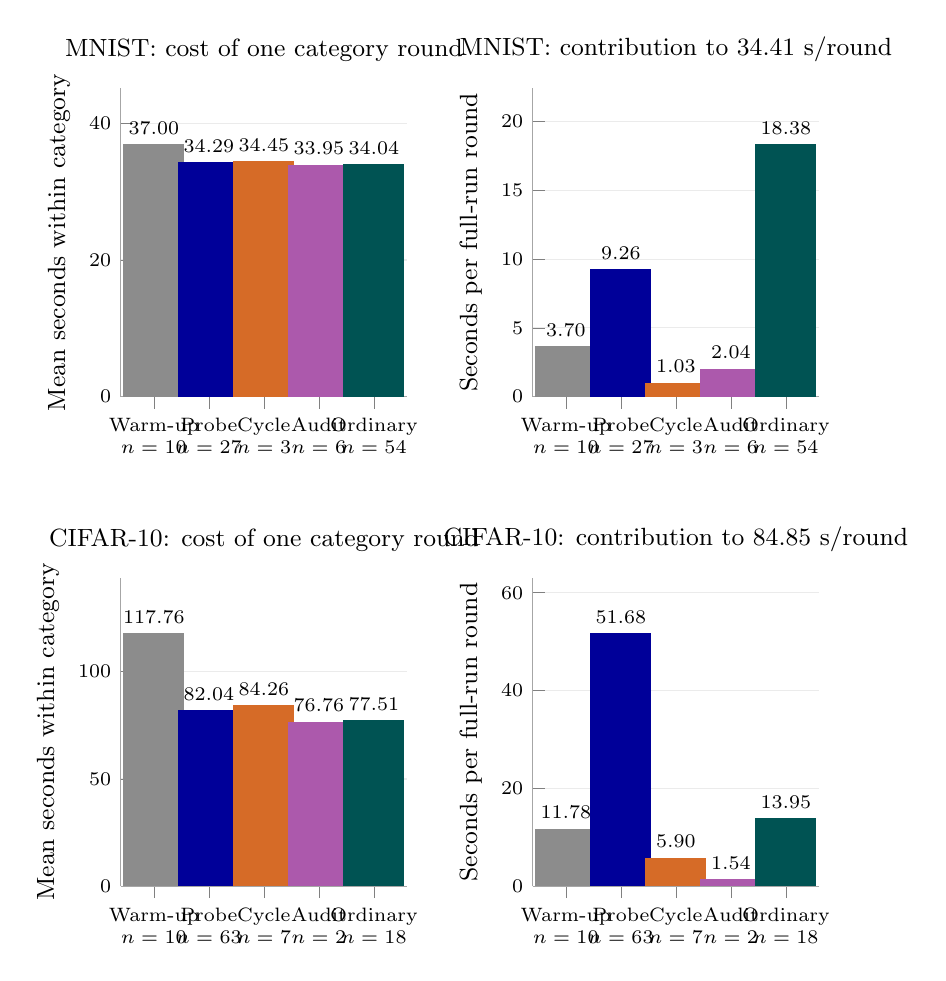
\begin{tikzpicture}
\begin{groupplot}[group style={group size=2 by 2,horizontal sep=1.6cm,vertical sep=2.3cm},
width=0.43\textwidth,height=5.5cm,
grid=major,grid style={black!8},axis line style={black!35},
tick label style={font=\scriptsize},label style={font=\small},title style={font=\small},
legend style={font=\scriptsize,draw=none},scaled y ticks=false]
\nextgroupplot[title={MNIST: cost of one category round},ybar,bar width=22pt,bar shift=0pt,ymin=0,ymax=45.135779,xmin=0.4,xmax=5.6,ylabel={Mean seconds within category},xtick={1,2,3,4,5},xticklabels={{Warm-up\\$n=10$},{Probe\\$n=27$},{Cycle\\$n=3$},{Audit\\$n=6$},{Ordinary\\$n=54$}},xticklabel style={align=center,font=\scriptsize},xmajorgrids=false,axis x line*=bottom,axis y line*=left,nodes near coords,every node near coord/.append style={font=\scriptsize,text=black,/pgf/number format/fixed,/pgf/number format/precision=2,/pgf/number format/fixed zerofill}]
\addplot[fill=black!45,draw=none,bar shift=0pt] coordinates {(1,36.996540260)};
\addplot[fill=blue!60!black,draw=none,bar shift=0pt] coordinates {(2,34.288500330)};
\addplot[fill=riderorange,draw=none,bar shift=0pt] coordinates {(3,34.450482100)};
\addplot[fill=violet!65,draw=none,bar shift=0pt] coordinates {(4,33.951632300)};
\addplot[fill=teal!65!black,draw=none,bar shift=0pt] coordinates {(5,34.036154717)};
\nextgroupplot[title={MNIST: contribution to 34.41 s/round},ybar,bar width=22pt,bar shift=0pt,ymin=0,ymax=22.423019,xmin=0.4,xmax=5.6,ylabel={Seconds per full-run round},xtick={1,2,3,4,5},xticklabels={{Warm-up\\$n=10$},{Probe\\$n=27$},{Cycle\\$n=3$},{Audit\\$n=6$},{Ordinary\\$n=54$}},xticklabel style={align=center,font=\scriptsize},xmajorgrids=false,axis x line*=bottom,axis y line*=left,nodes near coords,every node near coord/.append style={font=\scriptsize,text=black,/pgf/number format/fixed,/pgf/number format/precision=2,/pgf/number format/fixed zerofill}]
\addplot[fill=black!45,draw=none,bar shift=0pt] coordinates {(1,3.699654026)};
\addplot[fill=blue!60!black,draw=none,bar shift=0pt] coordinates {(2,9.257895089)};
\addplot[fill=riderorange,draw=none,bar shift=0pt] coordinates {(3,1.033514463)};
\addplot[fill=violet!65,draw=none,bar shift=0pt] coordinates {(4,2.037097938)};
\addplot[fill=teal!65!black,draw=none,bar shift=0pt] coordinates {(5,18.379523547)};
\nextgroupplot[title={CIFAR-10: cost of one category round},ybar,bar width=22pt,bar shift=0pt,ymin=0,ymax=143.668467,xmin=0.4,xmax=5.6,ylabel={Mean seconds within category},xtick={1,2,3,4,5},xticklabels={{Warm-up\\$n=10$},{Probe\\$n=63$},{Cycle\\$n=7$},{Audit\\$n=2$},{Ordinary\\$n=18$}},xticklabel style={align=center,font=\scriptsize},xmajorgrids=false,axis x line*=bottom,axis y line*=left,nodes near coords,every node near coord/.append style={font=\scriptsize,text=black,/pgf/number format/fixed,/pgf/number format/precision=2,/pgf/number format/fixed zerofill}]
\addplot[fill=black!45,draw=none,bar shift=0pt] coordinates {(1,117.761038190)};
\addplot[fill=blue!60!black,draw=none,bar shift=0pt] coordinates {(2,82.037953983)};
\addplot[fill=riderorange,draw=none,bar shift=0pt] coordinates {(3,84.261838643)};
\addplot[fill=violet!65,draw=none,bar shift=0pt] coordinates {(4,76.756039800)};
\addplot[fill=teal!65!black,draw=none,bar shift=0pt] coordinates {(5,77.510055911)};
\nextgroupplot[title={CIFAR-10: contribution to 84.85 s/round},ybar,bar width=22pt,bar shift=0pt,ymin=0,ymax=63.054371,xmin=0.4,xmax=5.6,ylabel={Seconds per full-run round},xtick={1,2,3,4,5},xticklabels={{Warm-up\\$n=10$},{Probe\\$n=63$},{Cycle\\$n=7$},{Audit\\$n=2$},{Ordinary\\$n=18$}},xticklabel style={align=center,font=\scriptsize},xmajorgrids=false,axis x line*=bottom,axis y line*=left,nodes near coords,every node near coord/.append style={font=\scriptsize,text=black,/pgf/number format/fixed,/pgf/number format/precision=2,/pgf/number format/fixed zerofill}]
\addplot[fill=black!45,draw=none,bar shift=0pt] coordinates {(1,11.776103819)};
\addplot[fill=blue!60!black,draw=none,bar shift=0pt] coordinates {(2,51.683911009)};
\addplot[fill=riderorange,draw=none,bar shift=0pt] coordinates {(3,5.898328705)};
\addplot[fill=violet!65,draw=none,bar shift=0pt] coordinates {(4,1.535120796)};
\addplot[fill=teal!65!black,draw=none,bar shift=0pt] coordinates {(5,13.951810064)};
\end{groupplot}\end{tikzpicture}
\caption{Where our 100-round runtime is spent (non-IID FR3, seed 42, 40\% free riders). Rows separate MNIST and CIFAR-10. Left: mean duration of a complete round in each category. Right: summed duration for that category divided by 100; the five bars add to the full-run mean printed in the title. Labels give category counts $n$. Probe excludes cycle-decision rounds; Cycle includes the final cycle decision; Audit is a single audit round. Categories are mutually exclusive. A cycle bar includes client training, aggregation and evaluation: it is NOT detector-only time. Axes scale independently; all bars start at zero.}\label{fig:timing-phases}
\end{figure*}

\begin{figure*}[tp]\centering\begin{tikzpicture}
\begin{groupplot}[group style={group size=2 by 1,horizontal sep=1.6cm,vertical sep=1.6cm},
width=0.43\textwidth,height=6.4cm,
grid=major,grid style={black!8},axis line style={black!35},
tick label style={font=\scriptsize},label style={font=\small},title style={font=\small},
legend style={font=\scriptsize,draw=none},scaled y ticks=false]
\nextgroupplot[title={MNIST},xmin=0,xmax=101,ymin=0,xlabel={Round},ylabel={Measured seconds},xtick={1,20,40,60,80,100},legend to name=timing-trace-legend,legend columns=3]
\addplot[black!65,thick] table[x=round,y=seconds] {\TimingDataDir/timeline_mnist.dat};
\addlegendentry{Ours: actual 100 rounds}
\addplot[only marks,mark=*,mark size=2pt,color=riderorange] table[x=round,y=seconds] {\TimingDataDir/cycle_rounds_mnist.dat};
\addlegendentry{Full-cycle decision rounds}
\addplot[blue!70!black,thick] table[x=round,y=seconds] {\TimingDataDir/std_rounds_mnist.dat};
\addlegendentry{STD: actual rounds 1--100}
\nextgroupplot[title={CIFAR-10},xmin=0,xmax=101,ymin=0,xlabel={Round},ylabel={Measured seconds},xtick={1,20,40,60,80,100}]
\addplot[black!65,thick] table[x=round,y=seconds] {\TimingDataDir/timeline_cifar10.dat};
\addplot[only marks,mark=*,mark size=2pt,color=riderorange] table[x=round,y=seconds] {\TimingDataDir/cycle_rounds_cifar10.dat};
\addplot[blue!70!black,thick] table[x=round,y=seconds] {\TimingDataDir/std_rounds_cifar10.dat};
\end{groupplot}\end{tikzpicture}
\par\ref{timing-trace-legend}
\caption{Actual per-round durations over 100 executed rounds for both methods. Our trajectories include changing active-client counts and probing schedules; STD-DAGMM retains all 100 clients. Markers indicate full-cycle decisions, not their isolated computational cost. Axis scales differ by dataset.}\label{fig:timing-traces}
\end{figure*}



\FloatBarrier
\section{Result Analysis}
\subsection{Effect of Attack Behavior}
\textbf{FR1} is consistently removed at the earliest allowed round. Exact
sendback provides a distinct evidence path, so its success does not validate
the statistical separation gate. Near-converged honest zero updates would
still require separate examination in other training regimes.

\textbf{FR2} is removed by round 30 in all settings despite avoiding equality.
The observed responses are sufficiently distinct under the configured random
update distribution and repeated traps. This is evidence about the tested
amplitude, not proof that arbitrary fabricated noise will be detected.

\textbf{FR3} is the critical heterogeneous-data case. Its current-inclusive
history can yield responses that overlap honest update geometry. In non-IID
CIFAR-10 at 40\% in the representative replication, all 40 free riders receive full norm certificates at rounds
20 and 60; at 30\%, all 30 receive them at rounds 40 and 80. Ambiguous intervening
cycles do not increment these counts. Retention permits the later fresh
certificate to confirm removal. This recorded sequence explains how the memory
rule operates; it is not a matched ablation proving that memory alone caused
the outcome under a counterfactual training trajectory.

\textbf{FR4} is removed by round 30 in the representative replication, while
additional replications require up to round \MultiCompletionMax{}. Its received-trajectory
estimate includes traps, which plausibly contributes to separation from genuine
optimization. This is an interpretation of the mechanism, not a measurement of
the attacker's inference ability. A defense-aware attacker could treat repeated
or unusual received states differently and needs a separate evaluation.

\subsection{Dataset, Partition, and Attacker Share}
MNIST FR1 to FR3 complete free-rider removal at round 30, while some MNIST FR4
and non-IID CIFAR-10 executions require additional evidence cycles. This shows that neither attack identity
alone nor final recall fully describes difficulty. The interaction between
honest-data heterogeneity, model state, and fabricated response geometry matters.

In the representative replication, changing the share from 40\% to 30\% preserves complete detection but delays
the difficult CIFAR-10 FR3 case from round 60 to round 80. A lower attacker
share therefore does not imply faster discovery. Cohort support and the
distribution of the surrounding honest population both change; the server does
not use the known simulation share to force a quota or boundary.

The 30\% runs also train 70 honest clients rather than 60. This increases
genuine local work and helps explain longer simulator round times without
implying a more expensive statistical rule. Non-IID client dataset sizes differ,
so the increase need not equal the 16.7\% change in honest-client count.
The slightly higher achieved accuracies at 30\% are consistent with more honest
training, but no causal effect is established without matched controls.

\subsection{Screening Quality Versus Removal Safety}
The evaluated procedure achieves high removal precision, but the additional
replications show that repeated evidence does not eliminate false positives.
The central unresolved issue is that some non-IID honest populations remain
almost entirely candidate-labelled after attackers disappear. This can arise
when relative statistical comparisons continue to find weak differences among
honest clients. Such labels do not, by themselves, exclude ordinary updates,
but they limit the meaning of calling R ``safe'' or C ``malicious.'' We interpret
R as unflagged, C as unresolved, and S as freshly certified suspicion.

Temporary exclusion also remains a real cost. Most honest exclusions are
deliberate trap responses, not quarantine. In ordinary successful MNIST runs,
660 honest client-rounds are withheld at 40\% and 770 at 30\%, corresponding
to eleven trap rounds per honest client over the 100-round horizon. The
exceptional FR3 follow-up adds further probing. A deployment should measure
whether this forgone aggregation delays reaching a target utility, rather
than reporting permanent-removal precision alone.

\subsection{What the Current Evidence Does Not Establish}
The repeated experiments assess variation across the tested seeds. Wider
validation should include honest-only populations, longer training horizons,
matched ablations, and baseline comparisons under identical trajectories.
Client observations within a run are correlated, and complete recall in these
experiments does not establish universal detection. Variations of attacker history length, noise
amplitude, trap strength, local epoch count, non-IID concentration, and model
architecture remain necessary robustness tests. In particular, the influence of
CIFAR BatchNorm buffers should be separated from trainable-weight evidence.

\section{Complexity and Lightweight Design}\label{sec:complexity}
\subsection{Operation Counts and Scaling}
Let $N$ be active clients, $P$ floating model coordinates (including floating
buffers), $L$ floating tensors, $T$ rounds, $B$ bootstrap replicates and
$K=\lceil\sqrt{N}\rceil$ histogram bins. The following are implementation
bounds, not measured wall-clock predictions. We count model scanning separately
from local optimization and ordinary aggregation.

\begin{table*}[t]\centering\footnotesize
\caption{Incremental detector operations and working state. ``Cycle'' means a complete A/B evidence cycle; it does not mean every training round. Bounds exclude ordinary model aggregation, local training, simulator attack histories and persistent logging.}\label{tab:complexity}
\begin{tabular}{p{3.6cm}p{3.6cm}p{3.0cm}p{5.3cm}}\toprule
Component & Work & Working state & Practical interpretation \\ \midrule
Norm, profile, exact fingerprint & $O(NP)$ per round & $O(P)$ scratch, $O(N)$ fingerprints & Sequential model reads; no auxiliary training or gradients. \\
Selected A/B summaries & $O(NL)$ per cycle to store & $O(NL)$ & Two compact profiles per active client, not full response histories. \\
Leave-one-out norm/profile scores & $O(N^2(L+\log N))$ per cycle & $O(NL)$ temporary & Repeated peer-profile medians/distances; Python scalar medians sort. \\
Three histogram/bootstrap views & $O(B(N+K))$ per cycle & $O(BN+BK)$ scratch & Three views add a constant factor; $B=1000$. \\
Geometric gates and memory & $O(N)$ selections/quantiles per cycle & $O(N)$ counters & Fixed component count; no learned detector or history-window reconstruction. \\
Two model challenges & $O(P)$ generation per cycle & $O(P)$ & Two shared trap states, not a distinct trap model per client. \\
\bottomrule\end{tabular}\end{table*}

The leave-one-out implementation rebuilds $N-1$ peer profiles for every
client and trap. Profile medians and distances require $O(N^2L)$ coordinate
work; repeated scalar medians in Python's \texttt{statistics.median} add
$O(N^2\log N)$ sorting work. Thus, calling the whole method linear in client
count would be incorrect. Histogram binning and bootstrap resampling operate
only on scalar scores, not on $P$-dimensional model vectors. With $M$ complete
cycles, the detector work is bounded by
\begin{equation}
\begin{aligned}
 W={}&O\bigl(TNP\bigr)\\
 &+O\!\left(M\left[N^2(L+\log N)+B(N+K)\right]\right).
\end{aligned}
\end{equation}
Single-trap audits add corresponding one-view scoring passes; they cannot
authorize permanent removal. Dense monitoring supplies more observations but
only one preselected A/B pair per client enters each complete-cycle decision.

At $N=100$, the two-trap profile comparison visits
$2N(N-1)L=158{,}400$ profile coordinates for MNIST and $435{,}600$ for CIFAR-10,
before constants for medians and distances. One bootstrap view draws $BN=100{,}000$
scalar indices; three views process three such sets using reused draws in the
current implementation. These counts explain why the evidence layer is compact
relative to repeated full-model training, but they do not measure its elapsed time.

\subsection{Payload Sizes, Memory Boundaries and Communication}
Table~\ref{tab:payload} derives concrete payload sizes from the implemented
architectures. The compact float32 pair payload is
$2N(L+3)\cdot4$ bytes under the stated packed representation; the three scalar
slots are an illustrative norm/round/flag allowance, not the actual Python object
layout. The two trap models occupy $2P\cdot4$ floating bytes. Actual dictionaries,
lists, Python scalars, allocator overhead, fingerprints and bootstrap temporaries
increase memory. For example, bootstrap index gathers and bin-index arrays coexist
with resample/count arrays; their two listed sizes must not be relabelled as peak
bootstrap RSS.
\begin{table*}[t]\centering\footnotesize
\caption{Calculated detector payload sizes at $N=100$, two traps, $B=1000$: architecture-derived estimates, NOT measured heap usage.}\label{tab:payload}
\begin{tabular}{lrrrrrrr}\toprule
Model & Parameters & $P$ & $L$ & Two traps (MiB) & Pair payload (KiB) & Index array (MiB) & Counts (MiB) \\ \midrule
MNIST & 206922 & 206922 & 8 & 1.579 & 8.594 & 0.763 & 0.076 \\
CIFAR-10 & 620810 & 621258 & 22 & 4.740 & 19.531 & 0.763 & 0.076 \\
\bottomrule\end{tabular}
\par\smallskip\begin{minipage}{0.96\textwidth}\scriptsize $P$ includes floating BatchNorm buffers; $L$ counts floating tensors. Pair payload assumes packed float32 profiles plus three scalar slots per trap/client. Bootstrap columns show two principal arrays, not peak scratch or an upper bound. No detector-only RSS was recorded.\end{minipage}\end{table*}


The decision working state is $O(P+NL+BN+BK)$, plus $O(N)$ counters and
fingerprints. In contrast, the research logger accumulates per-round/probe rows,
including tensor profiles, so the full simulator's retained evidence can grow
as $O(TNL)$ in dense probing. Ordinary aggregation also retains model responses,
and the simulator stores attack histories. The measured process RSS in
Table~\ref{tab:cost} includes these costs; it is not evidence that the entire
implementation uses only compact decision-state memory. Streaming logs and
aggregation would be deployment optimizations, not features benchmarked here.

No extra local optimization pass or auxiliary classifier is required. Under the
existing full-participation request/response schedule, traps replace ordinary
models rather than adding a second exchange; challenge responses are discarded
from aggregation. The nominal model-payload order remains $O(NP)$ per round,
excluding transport/serialization overhead. This does not make communication
``free'': useful contributions are withheld, so reaching a target accuracy can
require more rounds. Network-byte measurements and controlled detector-only
profiling are still necessary. We use \emph{lightweight} to mean compact features,
no auxiliary learning, and constant-sized per-client evidence memory, not an
unmeasured universal speed or energy advantage.

\section{Security Analysis}
\subsection{Decision Inputs and Attack-Label Separation}
The detector receives an allowlist of client/trap IDs, raw norms, profile
distances, robust scores, and exact-sendback indicators. The simulator's attacker
labels and behavior choices are not passed to screening, geometric tests, or
the client state machine. Evaluation prevalence determines how many attackers
the simulator creates, not how many removals the detector attempts to achieve.
This code boundary reduces direct evaluation leakage; it does not make the
development process independent of previously observed results.

\subsection{Confirmation Invariants}
Three operational safeguards follow from the state-transition rules.
First, statistical removal requires the same component on both selected traps
and a second distinct full cycle: one trap, mixed norm/profile evidence, or
an ambiguous result cannot independently supply the required confirmation.
Second, previously stored evidence does not authorize a new removal without
a fresh current certificate. Third, stored counts and weak C evidence cannot
renew quarantine; unconfirmed review expires unless fresh strong evidence
returns. These are protocol invariants, not probabilistic security bounds.

The guarantees are intentionally narrower than ``no false positives.'' An
honest client can satisfy the same geometric gate in two cycles. A clean
majority and independent trap draws do not make the resulting statistical
certificates independent, because clients retain the same data and related
model trajectories.

\subsection{Evasion, Identifiability, and Trap Secrecy}\label{sec:evasion}
Consider two executions with identical server-observable response histories,
public identities, and server randomness, one produced by honest training and
the other by fabrication. A detector whose transition function depends only on
those observations has the same state trajectory in both executions. Therefore,
update-only screening cannot prove genuine computation against every attacker.
The proposed method must be evaluated by how well its challenges separate
specified behaviors, not as a cryptographic proof of training.

The evaluated attackers are not given trap labels, but several real-world
signals could reveal auditing: repeated frozen states, abrupt distributional
changes, or communication between clients receiving different models. Moreover,
the simulator derives reproducible randomness from configured seeds; it does
not establish unpredictability against an adversary that knows those seeds.
Deployment would require server-secret randomness and an evaluation of
defense-aware response strategies. Even secret randomness alone would not
establish indistinguishability of traps from ordinary models.

\subsection{Honest-Client Safety and Long-Term Accumulation}
There is no fitted numerical z-score cutoff for statistical removal, but the
policy is not parameter-free. Trap scale, histogram binning, bootstrap confidence,
cohort support, confirmation count, and review/clearance lengths are design
choices. A stable boundary is not a calibrated false-removal probability.
At 100 clients the minimum statistical cohort support is ten; an isolated
nonzero free rider can therefore escape this cohort gate.

Certificate memory deliberately has no fixed age limit. If an honest client's
atypical geometry generates repeated strong evidence without two complete R
cycles, it can eventually be removed. The profile gate's concentration
alternative and persistent candidate populations make this a material
long-horizon risk. The honest removals observed in the repeated experiments
show that false evidence can lead to exclusion within 100 rounds. Longer
honest-only and heterogeneous-population experiments are
needed before making deployment safety claims.

\subsection{Privacy, Collusion, and Availability}
The protocol is not directly compatible with standard secure aggregation and
does not provide differential privacy~\cite{bonawitz2017practical}. Avoiding
client-reported loss and raw data access reduces required inputs but is not a
privacy proof: identifiable returned models may still leak information.
Colluding clients could share a genuinely trained response or infer the trap
schedule, and Sybil identities could distort the assumed honest-majority
reference. Neither attack is evaluated.

All active clients and complete A/B coverage are required for a certifying
cycle. Missing/nonfinite measurements cannot certify, and the current simulator
aborts on a nonfinite client response rather than implementing a complete
availability defense. Dropout tolerance, malicious-message handling, restart
integrity, authentication, and denial-of-service resistance require additional
engineering and experiments. Checkpoint recovery preserves computation and
evidence state after interruption; it does not create new evidence of honesty.

\subsection{Computational and Communication Exposure}
The bounds in Section~\ref{sec:complexity} expose quadratic-in-population
leave-one-out work and transient bootstrap memory. A large population or model
can make auditing expensive even without learned detector training. Deliberately
withheld trap responses and repeated honest follow-up are an availability and
utility cost, not merely an implementation detail. Communication bytes, time to
target utility, energy, and isolated detector work remain unmeasured.

\section{Conclusion}
This study evaluates a lightweight, server-observable challenge approach to
free-rider screening, with strict norm separation, component-specific evidence
memory, and bounded review. Evaluation across multiple random seeds on MNIST
and CIFAR-10 achieves \MultiRecall\% recall and pooled precision of
\MultiPrecision\%. Most executions complete detection by round 30, with more
difficult cases requiring up to round \MultiCompletionMax{}. The three honest
removals show that repeated confirmation does not eliminate false positives.
The results show useful separation under the evaluated
training and attack configurations, while the candidate and quarantine results
show why final recall and precision alone are insufficient.

Further validation should include broader client populations, honest-only
training, and tests of
adaptive/mixed attacks and longer horizons. Matched ablations and detector-only
profiling should distinguish the contributions of traps, geometric gates, and
memory from ordinary training and simulator costs. The method is a promising
empirical screening mechanism, not a universal verifier of local computation.

\FloatBarrier
\appendices
\section{Representative Per-Run Results}
Tables~\ref{tab:detail-mnist} and~\ref{tab:detail-cifar10} retain detailed outcomes
from the representative replication. Full records for the repeated experiments,
including the honest removals, are provided in
\path{generated/multiseed/per_run.csv}. Group means and accuracy standard
deviations are retained in \path{generated/multiseed/table1_means.csv}.
\begin{table*}[t]
\centering\footnotesize\setlength{\tabcolsep}{4pt}
\caption{Detection and utility outcomes for the representative MNIST replication.}\label{tab:detail-mnist}
\begin{tabular}{rllrrrrrrrr}
\toprule
FR (\%) & Partition & Attack & TP & FP & FN & $t_{\rm all}$ & Accuracy (\%) & $C_H$ & $Q_H$ & $q_H$ \\
\midrule
30 & IID & FR1 & 30 & 0 & 0 & 30 & 99.02 & 1 & 0 & 0 \\
30 & IID & FR2 & 30 & 0 & 0 & 30 & 99.00 & 5 & 0 & 0 \\
30 & IID & FR3 & 30 & 0 & 0 & 30 & 99.00 & 8 & 0 & 0 \\
30 & IID & FR4 & 30 & 0 & 0 & 30 & 98.82 & 2 & 0 & 0 \\
30 & Non-IID & FR1 & 30 & 0 & 0 & 30 & 99.01 & 7 & 0 & 0 \\
30 & Non-IID & FR2 & 30 & 0 & 0 & 30 & 99.00 & 6 & 0 & 0 \\
30 & Non-IID & FR3 & 30 & 0 & 0 & 30 & 98.98 & 8 & 0 & 0 \\
30 & Non-IID & FR4 & 30 & 0 & 0 & 30 & 98.96 & 6 & 0 & 0 \\
40 & IID & FR1 & 40 & 0 & 0 & 30 & 98.90 & 1 & 0 & 0 \\
40 & IID & FR2 & 40 & 0 & 0 & 30 & 98.91 & 5 & 0 & 0 \\
40 & IID & FR3 & 40 & 0 & 0 & 30 & 98.85 & 5 & 0 & 0 \\
40 & IID & FR4 & 40 & 0 & 0 & 30 & 98.77 & 5 & 0 & 0 \\
40 & Non-IID & FR1 & 40 & 0 & 0 & 30 & 98.96 & 2 & 0 & 0 \\
40 & Non-IID & FR2 & 40 & 0 & 0 & 30 & 98.96 & 7 & 0 & 0 \\
40 & Non-IID & FR3 & 40 & 0 & 0 & 30 & 98.93 & 34 & 1 & 20 \\
40 & Non-IID & FR4 & 40 & 0 & 0 & 30 & 98.98 & 12 & 0 & 0 \\
\bottomrule
\end{tabular}

\end{table*}

\begin{table*}[t]
\centering\footnotesize\setlength{\tabcolsep}{4pt}
\caption{Detection and utility outcomes for the representative CIFAR-10 replication.}\label{tab:detail-cifar10}
\begin{tabular}{rllrrrrrrrr}
\toprule
FR (\%) & Partition & Attack & TP & FP & FN & $t_{\rm all}$ & Accuracy (\%) & $C_H$ & $Q_H$ & $q_H$ \\
\midrule
30 & IID & FR1 & 30 & 0 & 0 & 30 & 78.07 & 2 & 0 & 0 \\
30 & IID & FR2 & 30 & 0 & 0 & 30 & 77.93 & 0 & 0 & 0 \\
30 & IID & FR3 & 30 & 0 & 0 & 30 & 78.17 & 2 & 0 & 0 \\
30 & IID & FR4 & 30 & 0 & 0 & 30 & 78.03 & 7 & 0 & 0 \\
30 & Non-IID & FR1 & 30 & 0 & 0 & 30 & 75.80 & 8 & 0 & 0 \\
30 & Non-IID & FR2 & 30 & 0 & 0 & 30 & 75.58 & 2 & 0 & 0 \\
30 & Non-IID & FR3 & 30 & 0 & 0 & 80 & 75.36 & 70 & 1 & 20 \\
30 & Non-IID & FR4 & 30 & 0 & 0 & 30 & 75.78 & 7 & 0 & 0 \\
40 & IID & FR1 & 40 & 0 & 0 & 30 & 77.46 & 0 & 0 & 0 \\
40 & IID & FR2 & 40 & 0 & 0 & 30 & 77.65 & 0 & 0 & 0 \\
40 & IID & FR3 & 40 & 0 & 0 & 30 & 77.27 & 4 & 0 & 0 \\
40 & IID & FR4 & 40 & 0 & 0 & 30 & 77.36 & 8 & 0 & 0 \\
40 & Non-IID & FR1 & 40 & 0 & 0 & 30 & 75.28 & 9 & 0 & 0 \\
40 & Non-IID & FR2 & 40 & 0 & 0 & 30 & 75.43 & 4 & 0 & 0 \\
40 & Non-IID & FR3 & 40 & 0 & 0 & 60 & 74.89 & 52 & 9 & 180 \\
40 & Non-IID & FR4 & 40 & 0 & 0 & 30 & 75.14 & 7 & 0 & 0 \\
\bottomrule
\end{tabular}

\end{table*}


\section{Supporting Trajectories and Score Geometry}\label{app:trajectories}
Figure~\ref{fig:recall} retains the representative cumulative detection trajectories, including
the delayed non-IID CIFAR-10 FR3 cases. Figure~\ref{fig:accuracy-overview} restores
the full training horizon and shared 0--1 scale for interpreting the main-text
accuracy zooms. Figures~\ref{fig:scatter-mnist-30} and
\ref{fig:scatter-cifar10-30} show the complementary 30\% client clouds using
the same paired-score definition and monotone display transformation.
\begin{figure*}[tp]\centering
\begin{tikzpicture}
\begin{groupplot}[group style={group size=2 by 4,horizontal sep=0.9cm,vertical sep=1.25cm},
width=0.455\textwidth,height=4.6cm,xmin=0,xmax=100,
ymin=0,ymax=1.05,
grid=major,xtick={0,30,60,100},tick label style={font=\scriptsize},
title style={font=\small},label style={font=\scriptsize},legend style={font=\scriptsize,draw=none},
legend columns=4]
\nextgroupplot[title={MNIST FR1},ylabel={Removal recall},legend to name=fig:recall-legend]
\addplot[blue,solid,thick,const plot] table[x=round,y=recall] {generated/mnist_iid_FR1_p30.dat};
\addlegendentry{30\% IID}
\addplot[red!80!black,dashed,thick,const plot] table[x=round,y=recall] {generated/mnist_noniid_FR1_p30.dat};
\addlegendentry{30\% Non-IID}
\addplot[teal!70!black,dotted,thick,const plot] table[x=round,y=recall] {generated/mnist_iid_FR1_p40.dat};
\addlegendentry{40\% IID}
\addplot[orange!90!black,dashdotted,thick,const plot] table[x=round,y=recall] {generated/mnist_noniid_FR1_p40.dat};
\addlegendentry{40\% Non-IID}
\nextgroupplot[title={MNIST FR2}]
\addplot[blue,solid,thick,const plot] table[x=round,y=recall] {generated/mnist_iid_FR2_p30.dat};
\addplot[red!80!black,dashed,thick,const plot] table[x=round,y=recall] {generated/mnist_noniid_FR2_p30.dat};
\addplot[teal!70!black,dotted,thick,const plot] table[x=round,y=recall] {generated/mnist_iid_FR2_p40.dat};
\addplot[orange!90!black,dashdotted,thick,const plot] table[x=round,y=recall] {generated/mnist_noniid_FR2_p40.dat};
\nextgroupplot[title={MNIST FR3}]
\addplot[blue,solid,thick,const plot] table[x=round,y=recall] {generated/mnist_iid_FR3_p30.dat};
\addplot[red!80!black,dashed,thick,const plot] table[x=round,y=recall] {generated/mnist_noniid_FR3_p30.dat};
\addplot[teal!70!black,dotted,thick,const plot] table[x=round,y=recall] {generated/mnist_iid_FR3_p40.dat};
\addplot[orange!90!black,dashdotted,thick,const plot] table[x=round,y=recall] {generated/mnist_noniid_FR3_p40.dat};
\nextgroupplot[title={MNIST FR4}]
\addplot[blue,solid,thick,const plot] table[x=round,y=recall] {generated/mnist_iid_FR4_p30.dat};
\addplot[red!80!black,dashed,thick,const plot] table[x=round,y=recall] {generated/mnist_noniid_FR4_p30.dat};
\addplot[teal!70!black,dotted,thick,const plot] table[x=round,y=recall] {generated/mnist_iid_FR4_p40.dat};
\addplot[orange!90!black,dashdotted,thick,const plot] table[x=round,y=recall] {generated/mnist_noniid_FR4_p40.dat};
\nextgroupplot[title={CIFAR-10 FR1},ylabel={Removal recall}]
\addplot[blue,solid,thick,const plot] table[x=round,y=recall] {generated/cifar10_iid_FR1_p30.dat};
\addplot[red!80!black,dashed,thick,const plot] table[x=round,y=recall] {generated/cifar10_noniid_FR1_p30.dat};
\addplot[teal!70!black,dotted,thick,const plot] table[x=round,y=recall] {generated/cifar10_iid_FR1_p40.dat};
\addplot[orange!90!black,dashdotted,thick,const plot] table[x=round,y=recall] {generated/cifar10_noniid_FR1_p40.dat};
\nextgroupplot[title={CIFAR-10 FR2}]
\addplot[blue,solid,thick,const plot] table[x=round,y=recall] {generated/cifar10_iid_FR2_p30.dat};
\addplot[red!80!black,dashed,thick,const plot] table[x=round,y=recall] {generated/cifar10_noniid_FR2_p30.dat};
\addplot[teal!70!black,dotted,thick,const plot] table[x=round,y=recall] {generated/cifar10_iid_FR2_p40.dat};
\addplot[orange!90!black,dashdotted,thick,const plot] table[x=round,y=recall] {generated/cifar10_noniid_FR2_p40.dat};
\nextgroupplot[title={CIFAR-10 FR3},xlabel={Round}]
\addplot[blue,solid,thick,const plot] table[x=round,y=recall] {generated/cifar10_iid_FR3_p30.dat};
\addplot[red!80!black,dashed,thick,const plot] table[x=round,y=recall] {generated/cifar10_noniid_FR3_p30.dat};
\addplot[teal!70!black,dotted,thick,const plot] table[x=round,y=recall] {generated/cifar10_iid_FR3_p40.dat};
\addplot[orange!90!black,dashdotted,thick,const plot] table[x=round,y=recall] {generated/cifar10_noniid_FR3_p40.dat};
\nextgroupplot[title={CIFAR-10 FR4},xlabel={Round}]
\addplot[blue,solid,thick,const plot] table[x=round,y=recall] {generated/cifar10_iid_FR4_p30.dat};
\addplot[red!80!black,dashed,thick,const plot] table[x=round,y=recall] {generated/cifar10_noniid_FR4_p30.dat};
\addplot[teal!70!black,dotted,thick,const plot] table[x=round,y=recall] {generated/cifar10_iid_FR4_p40.dat};
\addplot[orange!90!black,dashdotted,thick,const plot] table[x=round,y=recall] {generated/cifar10_noniid_FR4_p40.dat};
\end{groupplot}\end{tikzpicture}
\par\ref{fig:recall-legend}
\caption{Cumulative free-rider removal recall in the representative replication. Enlarged two-column panels identify dataset and attack in each title; the four lines distinguish partition and attacker share. Coincident curves overlap. Complete outcomes are retained, including incomplete detection if present.}\label{fig:recall}
\end{figure*}

\begin{figure*}[tp]\centering
\begin{tikzpicture}
\begin{groupplot}[group style={group size=2 by 4,horizontal sep=0.9cm,vertical sep=1.25cm},
width=0.455\textwidth,height=4.6cm,xmin=0,xmax=100,
ymin=0,ymax=1.02,
grid=major,xtick={0,30,60,100},tick label style={font=\scriptsize},
title style={font=\small},label style={font=\scriptsize},legend style={font=\scriptsize,draw=none},
legend columns=4]
\nextgroupplot[title={MNIST FR1},ylabel={Test accuracy},legend to name=fig:accuracy-overview-legend]
\addplot[blue,solid,thick] table[x=round,y=accuracy] {generated/mnist_iid_FR1_p30.dat};
\addlegendentry{30\% IID}
\addplot[red!80!black,dashed,thick] table[x=round,y=accuracy] {generated/mnist_noniid_FR1_p30.dat};
\addlegendentry{30\% Non-IID}
\addplot[teal!70!black,dotted,thick] table[x=round,y=accuracy] {generated/mnist_iid_FR1_p40.dat};
\addlegendentry{40\% IID}
\addplot[orange!90!black,dashdotted,thick] table[x=round,y=accuracy] {generated/mnist_noniid_FR1_p40.dat};
\addlegendentry{40\% Non-IID}
\nextgroupplot[title={MNIST FR2}]
\addplot[blue,solid,thick] table[x=round,y=accuracy] {generated/mnist_iid_FR2_p30.dat};
\addplot[red!80!black,dashed,thick] table[x=round,y=accuracy] {generated/mnist_noniid_FR2_p30.dat};
\addplot[teal!70!black,dotted,thick] table[x=round,y=accuracy] {generated/mnist_iid_FR2_p40.dat};
\addplot[orange!90!black,dashdotted,thick] table[x=round,y=accuracy] {generated/mnist_noniid_FR2_p40.dat};
\nextgroupplot[title={MNIST FR3}]
\addplot[blue,solid,thick] table[x=round,y=accuracy] {generated/mnist_iid_FR3_p30.dat};
\addplot[red!80!black,dashed,thick] table[x=round,y=accuracy] {generated/mnist_noniid_FR3_p30.dat};
\addplot[teal!70!black,dotted,thick] table[x=round,y=accuracy] {generated/mnist_iid_FR3_p40.dat};
\addplot[orange!90!black,dashdotted,thick] table[x=round,y=accuracy] {generated/mnist_noniid_FR3_p40.dat};
\nextgroupplot[title={MNIST FR4}]
\addplot[blue,solid,thick] table[x=round,y=accuracy] {generated/mnist_iid_FR4_p30.dat};
\addplot[red!80!black,dashed,thick] table[x=round,y=accuracy] {generated/mnist_noniid_FR4_p30.dat};
\addplot[teal!70!black,dotted,thick] table[x=round,y=accuracy] {generated/mnist_iid_FR4_p40.dat};
\addplot[orange!90!black,dashdotted,thick] table[x=round,y=accuracy] {generated/mnist_noniid_FR4_p40.dat};
\nextgroupplot[title={CIFAR-10 FR1},ylabel={Test accuracy}]
\addplot[blue,solid,thick] table[x=round,y=accuracy] {generated/cifar10_iid_FR1_p30.dat};
\addplot[red!80!black,dashed,thick] table[x=round,y=accuracy] {generated/cifar10_noniid_FR1_p30.dat};
\addplot[teal!70!black,dotted,thick] table[x=round,y=accuracy] {generated/cifar10_iid_FR1_p40.dat};
\addplot[orange!90!black,dashdotted,thick] table[x=round,y=accuracy] {generated/cifar10_noniid_FR1_p40.dat};
\nextgroupplot[title={CIFAR-10 FR2}]
\addplot[blue,solid,thick] table[x=round,y=accuracy] {generated/cifar10_iid_FR2_p30.dat};
\addplot[red!80!black,dashed,thick] table[x=round,y=accuracy] {generated/cifar10_noniid_FR2_p30.dat};
\addplot[teal!70!black,dotted,thick] table[x=round,y=accuracy] {generated/cifar10_iid_FR2_p40.dat};
\addplot[orange!90!black,dashdotted,thick] table[x=round,y=accuracy] {generated/cifar10_noniid_FR2_p40.dat};
\nextgroupplot[title={CIFAR-10 FR3},xlabel={Round}]
\addplot[blue,solid,thick] table[x=round,y=accuracy] {generated/cifar10_iid_FR3_p30.dat};
\addplot[red!80!black,dashed,thick] table[x=round,y=accuracy] {generated/cifar10_noniid_FR3_p30.dat};
\addplot[teal!70!black,dotted,thick] table[x=round,y=accuracy] {generated/cifar10_iid_FR3_p40.dat};
\addplot[orange!90!black,dashdotted,thick] table[x=round,y=accuracy] {generated/cifar10_noniid_FR3_p40.dat};
\nextgroupplot[title={CIFAR-10 FR4},xlabel={Round}]
\addplot[blue,solid,thick] table[x=round,y=accuracy] {generated/cifar10_iid_FR4_p30.dat};
\addplot[red!80!black,dashed,thick] table[x=round,y=accuracy] {generated/cifar10_noniid_FR4_p30.dat};
\addplot[teal!70!black,dotted,thick] table[x=round,y=accuracy] {generated/cifar10_iid_FR4_p40.dat};
\addplot[orange!90!black,dashdotted,thick] table[x=round,y=accuracy] {generated/cifar10_noniid_FR4_p40.dat};
\end{groupplot}\end{tikzpicture}
\par\ref{fig:accuracy-overview-legend}
\caption{Full, unzoomed global test-accuracy trajectories for the representative replication, providing context for the late-training detail in the main text.}\label{fig:accuracy-overview}
\end{figure*}

\begin{figure*}[tp]\centering
\begin{tikzpicture}
\begin{groupplot}[group style={group size=2 by 4,horizontal sep=0.8cm,vertical sep=1.25cm},
width=0.455\textwidth,height=4.6cm,
axis line style={black!35},grid=major,grid style={black!8},
tick label style={font=\scriptsize},title style={font=\small},
label style={font=\scriptsize},legend style={font=\scriptsize,draw=none},
scaled ticks=false,unbounded coords=jump]
\nextgroupplot[title={IID FR1},ylabel={$\operatorname{asinh}(\bar z_{\rm profile})$},legend to name=scatter-mnist-30-legend,legend columns=2]
\addplot[only marks,mark=o,mark size=1.65pt,color=honestblue,opacity=0.7] table[x=x,y=y] {generated/visuals/scatter_mnist_30_iid_FR1_0.dat};
\addlegendentry{Honest}
\addplot[only marks,mark=triangle*,mark size=1.65pt,color=riderorange,opacity=0.7] table[x=x,y=y] {generated/visuals/scatter_mnist_30_iid_FR1_1.dat};
\addlegendentry{Free rider}
\nextgroupplot[title={IID FR2},]
\addplot[only marks,mark=o,mark size=1.65pt,color=honestblue,opacity=0.7] table[x=x,y=y] {generated/visuals/scatter_mnist_30_iid_FR2_0.dat};
\addplot[only marks,mark=triangle*,mark size=1.65pt,color=riderorange,opacity=0.7] table[x=x,y=y] {generated/visuals/scatter_mnist_30_iid_FR2_1.dat};
\nextgroupplot[title={IID FR3},ylabel={$\operatorname{asinh}(\bar z_{\rm profile})$}]
\addplot[only marks,mark=o,mark size=1.65pt,color=honestblue,opacity=0.7] table[x=x,y=y] {generated/visuals/scatter_mnist_30_iid_FR3_0.dat};
\addplot[only marks,mark=triangle*,mark size=1.65pt,color=riderorange,opacity=0.7] table[x=x,y=y] {generated/visuals/scatter_mnist_30_iid_FR3_1.dat};
\nextgroupplot[title={IID FR4},]
\addplot[only marks,mark=o,mark size=1.65pt,color=honestblue,opacity=0.7] table[x=x,y=y] {generated/visuals/scatter_mnist_30_iid_FR4_0.dat};
\addplot[only marks,mark=triangle*,mark size=1.65pt,color=riderorange,opacity=0.7] table[x=x,y=y] {generated/visuals/scatter_mnist_30_iid_FR4_1.dat};
\nextgroupplot[title={Non-IID FR1},ylabel={$\operatorname{asinh}(\bar z_{\rm profile})$}]
\addplot[only marks,mark=o,mark size=1.65pt,color=honestblue,opacity=0.7] table[x=x,y=y] {generated/visuals/scatter_mnist_30_noniid_FR1_0.dat};
\addplot[only marks,mark=triangle*,mark size=1.65pt,color=riderorange,opacity=0.7] table[x=x,y=y] {generated/visuals/scatter_mnist_30_noniid_FR1_1.dat};
\nextgroupplot[title={Non-IID FR2},]
\addplot[only marks,mark=o,mark size=1.65pt,color=honestblue,opacity=0.7] table[x=x,y=y] {generated/visuals/scatter_mnist_30_noniid_FR2_0.dat};
\addplot[only marks,mark=triangle*,mark size=1.65pt,color=riderorange,opacity=0.7] table[x=x,y=y] {generated/visuals/scatter_mnist_30_noniid_FR2_1.dat};
\nextgroupplot[title={Non-IID FR3},xlabel={$\operatorname{asinh}(\bar z_{\rm norm})$},ylabel={$\operatorname{asinh}(\bar z_{\rm profile})$}]
\addplot[only marks,mark=o,mark size=1.65pt,color=honestblue,opacity=0.7] table[x=x,y=y] {generated/visuals/scatter_mnist_30_noniid_FR3_0.dat};
\addplot[only marks,mark=triangle*,mark size=1.65pt,color=riderorange,opacity=0.7] table[x=x,y=y] {generated/visuals/scatter_mnist_30_noniid_FR3_1.dat};
\nextgroupplot[title={Non-IID FR4},xlabel={$\operatorname{asinh}(\bar z_{\rm norm})$}]
\addplot[only marks,mark=o,mark size=1.65pt,color=honestblue,opacity=0.7] table[x=x,y=y] {generated/visuals/scatter_mnist_30_noniid_FR4_0.dat};
\addplot[only marks,mark=triangle*,mark size=1.65pt,color=riderorange,opacity=0.7] table[x=x,y=y] {generated/visuals/scatter_mnist_30_noniid_FR4_1.dat};
\end{groupplot}\end{tikzpicture}
\par\ref{scatter-mnist-30-legend}
\caption{MNIST: round-20 score geometry at 30\% free riders (all eight settings). One point is one client, averaging the A/B norm-z and profile-z scores separately. The monotone asinh display compresses extreme tails without clipping; zero remains zero, but distances are transformed. Panels autoscale independently. Labels color evaluation only, never references or decisions. 0 points have undefined coordinates and are omitted; coincident points overlap. No plotted line is a removal cutoff.}\label{fig:scatter-mnist-30}
\end{figure*}

\begin{figure*}[tp]\centering
\begin{tikzpicture}
\begin{groupplot}[group style={group size=2 by 4,horizontal sep=0.8cm,vertical sep=1.25cm},
width=0.455\textwidth,height=4.6cm,
axis line style={black!35},grid=major,grid style={black!8},
tick label style={font=\scriptsize},title style={font=\small},
label style={font=\scriptsize},legend style={font=\scriptsize,draw=none},
scaled ticks=false,unbounded coords=jump]
\nextgroupplot[title={IID FR1},ylabel={$\operatorname{asinh}(\bar z_{\rm profile})$},legend to name=scatter-cifar10-30-legend,legend columns=2]
\addplot[only marks,mark=o,mark size=1.65pt,color=honestblue,opacity=0.7] table[x=x,y=y] {generated/visuals/scatter_cifar10_30_iid_FR1_0.dat};
\addlegendentry{Honest}
\addplot[only marks,mark=triangle*,mark size=1.65pt,color=riderorange,opacity=0.7] table[x=x,y=y] {generated/visuals/scatter_cifar10_30_iid_FR1_1.dat};
\addlegendentry{Free rider}
\nextgroupplot[title={IID FR2},]
\addplot[only marks,mark=o,mark size=1.65pt,color=honestblue,opacity=0.7] table[x=x,y=y] {generated/visuals/scatter_cifar10_30_iid_FR2_0.dat};
\addplot[only marks,mark=triangle*,mark size=1.65pt,color=riderorange,opacity=0.7] table[x=x,y=y] {generated/visuals/scatter_cifar10_30_iid_FR2_1.dat};
\nextgroupplot[title={IID FR3},ylabel={$\operatorname{asinh}(\bar z_{\rm profile})$}]
\addplot[only marks,mark=o,mark size=1.65pt,color=honestblue,opacity=0.7] table[x=x,y=y] {generated/visuals/scatter_cifar10_30_iid_FR3_0.dat};
\addplot[only marks,mark=triangle*,mark size=1.65pt,color=riderorange,opacity=0.7] table[x=x,y=y] {generated/visuals/scatter_cifar10_30_iid_FR3_1.dat};
\nextgroupplot[title={IID FR4},]
\addplot[only marks,mark=o,mark size=1.65pt,color=honestblue,opacity=0.7] table[x=x,y=y] {generated/visuals/scatter_cifar10_30_iid_FR4_0.dat};
\addplot[only marks,mark=triangle*,mark size=1.65pt,color=riderorange,opacity=0.7] table[x=x,y=y] {generated/visuals/scatter_cifar10_30_iid_FR4_1.dat};
\nextgroupplot[title={Non-IID FR1},ylabel={$\operatorname{asinh}(\bar z_{\rm profile})$}]
\addplot[only marks,mark=o,mark size=1.65pt,color=honestblue,opacity=0.7] table[x=x,y=y] {generated/visuals/scatter_cifar10_30_noniid_FR1_0.dat};
\addplot[only marks,mark=triangle*,mark size=1.65pt,color=riderorange,opacity=0.7] table[x=x,y=y] {generated/visuals/scatter_cifar10_30_noniid_FR1_1.dat};
\nextgroupplot[title={Non-IID FR2},]
\addplot[only marks,mark=o,mark size=1.65pt,color=honestblue,opacity=0.7] table[x=x,y=y] {generated/visuals/scatter_cifar10_30_noniid_FR2_0.dat};
\addplot[only marks,mark=triangle*,mark size=1.65pt,color=riderorange,opacity=0.7] table[x=x,y=y] {generated/visuals/scatter_cifar10_30_noniid_FR2_1.dat};
\nextgroupplot[title={Non-IID FR3},xlabel={$\operatorname{asinh}(\bar z_{\rm norm})$},ylabel={$\operatorname{asinh}(\bar z_{\rm profile})$}]
\addplot[only marks,mark=o,mark size=1.65pt,color=honestblue,opacity=0.7] table[x=x,y=y] {generated/visuals/scatter_cifar10_30_noniid_FR3_0.dat};
\addplot[only marks,mark=triangle*,mark size=1.65pt,color=riderorange,opacity=0.7] table[x=x,y=y] {generated/visuals/scatter_cifar10_30_noniid_FR3_1.dat};
\nextgroupplot[title={Non-IID FR4},xlabel={$\operatorname{asinh}(\bar z_{\rm norm})$}]
\addplot[only marks,mark=o,mark size=1.65pt,color=honestblue,opacity=0.7] table[x=x,y=y] {generated/visuals/scatter_cifar10_30_noniid_FR4_0.dat};
\addplot[only marks,mark=triangle*,mark size=1.65pt,color=riderorange,opacity=0.7] table[x=x,y=y] {generated/visuals/scatter_cifar10_30_noniid_FR4_1.dat};
\end{groupplot}\end{tikzpicture}
\par\ref{scatter-cifar10-30-legend}
\caption{CIFAR-10: round-20 score geometry at 30\% free riders (all eight settings). One point is one client, averaging the A/B norm-z and profile-z scores separately. The monotone asinh display compresses extreme tails without clipping; zero remains zero, but distances are transformed. Panels autoscale independently. Labels color evaluation only, never references or decisions. 0 points have undefined coordinates and are omitted; coincident points overlap. No plotted line is a removal cutoff.}\label{fig:scatter-cifar10-30}
\end{figure*}


\section{Reproducibility and Interpretation Notes}
Table~\ref{tab:performance} is generated by
\path{build_multiseed_table.ps1}. It validates completion markers, configuration
coverage, training rounds, initial A/B coverage, removal identities and timing,
summary counts, final accuracy, detector policy, and six recorded implementation
hashes across all replications. Seed identifiers and input hashes are retained
in \path{generated/multiseed/provenance.json}, with individual outcomes and
grouped means in the accompanying CSV files. These records include failed
detections and honest removals rather than selecting only favorable outcomes.

The representative diagnostic assets are retained from the earlier development
replication. Their input hashes are recorded in
\path{generated/provenance.json}, and the six matching source files are copied
to \path{evidence/source/}. These hashes describe the recorded implementation
and do not attest the complete historical environment.
The score exports retain raw paired coordinates and per-class means, medians,
quartiles, finite counts and undefined counts for every complete evidence cycle.
Additional resource-comparison inputs and the architecture hash are recorded in
\texttt{generated/visual\_provenance.json}. The historical v15.3 cost table is
separate context and is never pooled with v15.4 detection totals.

The diagnostic tables and figures are preserved from v6, with captions updated
to distinguish individual executions from the averages in
Table~\ref{tab:performance}. Compile \texttt{paper\_v7.tex} with PDFLaTeX and BibTeX, or
use the accompanying \texttt{build.ps1}. Previous paper versions and all
experiment logs remain unchanged.
The older v2/v8 results are not pooled with the current method: in particular,
FR1 semantics, confirmation, reference construction, and screening policy differ.

Interrupted runs resume their last published checkpoint with loader/RNG state,
attack histories, selected probe positions, quarantine and confirmation memory.
The runtime table reports logged execution measures rather than powered-off
calendar waiting. None of the reported resource values should be relabelled as
detector-only overhead or interpreted as evidence of privacy/security guarantees.

\FloatBarrier
\bibliographystyle{IEEEtran}
\bibliography{refs}
\end{document}
